\documentclass{book}
\usepackage[a4paper,top=2.5cm,bottom=2.5cm,left=2.5cm,right=2.5cm]{geometry}
\usepackage{makeidx}
\usepackage{natbib}
\usepackage{graphicx}
\usepackage{multicol}
\usepackage{float}
\usepackage{listings}
\usepackage{color}
\usepackage{ifthen}
\usepackage[table]{xcolor}
\usepackage{textcomp}
\usepackage{alltt}
\usepackage{ifpdf}
\ifpdf
\usepackage[pdftex,
            pagebackref=true,
            colorlinks=true,
            linkcolor=blue,
            unicode
           ]{hyperref}
\else
\usepackage[ps2pdf,
            pagebackref=true,
            colorlinks=true,
            linkcolor=blue,
            unicode
           ]{hyperref}
\usepackage{pspicture}
\fi
\usepackage[utf8]{inputenc}
\usepackage{mathptmx}
\usepackage[scaled=.90]{helvet}
\usepackage{courier}
\usepackage{sectsty}
\usepackage[titles]{tocloft}
\usepackage{doxygen}
\lstset{language=C++,inputencoding=utf8,basicstyle=\footnotesize,breaklines=true,breakatwhitespace=true,tabsize=8,numbers=left }
\makeindex
\setcounter{tocdepth}{3}
\renewcommand{\footrulewidth}{0.4pt}
\renewcommand{\familydefault}{\sfdefault}
\hfuzz=15pt
\setlength{\emergencystretch}{15pt}
\hbadness=750
\tolerance=750
\begin{document}
\hypersetup{pageanchor=false,citecolor=blue}
\begin{titlepage}
\vspace*{7cm}
\begin{center}
{\Large V\-A\-S\-T }\\
\vspace*{1cm}
{\large Generated by Doxygen 1.8.1.1}\\
\vspace*{0.5cm}
{\small Tue Jun 12 2012 00:19:39}\\
\end{center}
\end{titlepage}
\clearemptydoublepage
\pagenumbering{roman}
\tableofcontents
\clearemptydoublepage
\pagenumbering{arabic}
\hypersetup{pageanchor=true,citecolor=blue}
\chapter{Class Index}
\section{Class Hierarchy}
This inheritance list is sorted roughly, but not completely, alphabetically\-:\begin{DoxyCompactList}
\item \contentsline{section}{A\-R\-Astar\-Heap}{\pageref{class_a_r_astar_heap}}{}
\item \contentsline{section}{A\-R\-Astar\-Heap\-Node}{\pageref{class_a_r_astar_heap_node}}{}
\item \contentsline{section}{A\-R\-Astar\-Node}{\pageref{class_a_r_astar_node}}{}
\item \contentsline{section}{A\-R\-Astar\-Planner}{\pageref{class_a_r_astar_planner}}{}
\item \contentsline{section}{A\-R\-Astar\-Test}{\pageref{class_a_r_astar_test}}{}
\item \contentsline{section}{Best\-First\-Search\-Node}{\pageref{class_best_first_search_node}}{}
\item \contentsline{section}{Best\-First\-Search\-Planner}{\pageref{class_best_first_search_planner}}{}
\item \contentsline{section}{Best\-First\-Search\-Test}{\pageref{class_best_first_search_test}}{}
\item \contentsline{section}{Close\-Container}{\pageref{class_close_container}}{}
\item \contentsline{section}{Compare\-Costs}{\pageref{class_compare_costs}}{}
\item \contentsline{section}{Default\-Action}{\pageref{class_default_action}}{}
\begin{DoxyCompactList}
\item \contentsline{section}{A\-R\-Astar\-Action}{\pageref{class_a_r_astar_action}}{}
\item \contentsline{section}{Best\-First\-Action}{\pageref{class_best_first_action}}{}
\end{DoxyCompactList}
\item \contentsline{section}{Default\-State}{\pageref{class_default_state}}{}
\begin{DoxyCompactList}
\item \contentsline{section}{A\-R\-Astar\-State}{\pageref{class_a_r_astar_state}}{}
\item \contentsline{section}{Best\-First\-State}{\pageref{class_best_first_state}}{}
\end{DoxyCompactList}
\item \contentsline{section}{Incons}{\pageref{class_incons}}{}
\item \contentsline{section}{I\-Planner\-Interface$<$ State\-Map $>$}{\pageref{interface_i_planner_interface-g}}{}
\item \contentsline{section}{Neighbor\-Map}{\pageref{class_neighbor_map}}{}
\begin{DoxyCompactList}
\item \contentsline{section}{Grid\-Neighbors}{\pageref{class_grid_neighbors}}{}
\end{DoxyCompactList}
\item \contentsline{section}{Node\-Comparer}{\pageref{class_node_comparer}}{}
\item \contentsline{section}{Open\-Container}{\pageref{class_open_container}}{}
\item \contentsline{section}{Plan\-Container}{\pageref{class_plan_container}}{}
\item \contentsline{section}{Planner}{\pageref{class_planner}}{}
\item \contentsline{section}{Planning\-Domain\-Base}{\pageref{class_planning_domain_base}}{}
\begin{DoxyCompactList}
\item \contentsline{section}{A\-R\-Astar\-Domain}{\pageref{class_a_r_astar_domain}}{}
\item \contentsline{section}{Best\-First\-Domain}{\pageref{class_best_first_domain}}{}
\end{DoxyCompactList}
\end{DoxyCompactList}

\chapter{Class Index}
\section{Class List}
Here are the classes, structs, unions and interfaces with brief descriptions\-:\begin{DoxyCompactList}
\item\contentsline{section}{\hyperlink{class_a_r_astar_action}{A\-R\-Astar\-Action} }{\pageref{class_a_r_astar_action}}{}
\item\contentsline{section}{\hyperlink{class_a_r_astar_domain}{A\-R\-Astar\-Domain} }{\pageref{class_a_r_astar_domain}}{}
\item\contentsline{section}{\hyperlink{class_a_r_astar_heap}{A\-R\-Astar\-Heap} }{\pageref{class_a_r_astar_heap}}{}
\item\contentsline{section}{\hyperlink{class_a_r_astar_heap_node}{A\-R\-Astar\-Heap\-Node} }{\pageref{class_a_r_astar_heap_node}}{}
\item\contentsline{section}{\hyperlink{class_a_r_astar_node}{A\-R\-Astar\-Node} }{\pageref{class_a_r_astar_node}}{}
\item\contentsline{section}{\hyperlink{class_a_r_astar_planner}{A\-R\-Astar\-Planner} }{\pageref{class_a_r_astar_planner}}{}
\item\contentsline{section}{\hyperlink{class_a_r_astar_state}{A\-R\-Astar\-State} }{\pageref{class_a_r_astar_state}}{}
\item\contentsline{section}{\hyperlink{class_a_r_astar_test}{A\-R\-Astar\-Test} }{\pageref{class_a_r_astar_test}}{}
\item\contentsline{section}{\hyperlink{class_best_first_action}{Best\-First\-Action} }{\pageref{class_best_first_action}}{}
\item\contentsline{section}{\hyperlink{class_best_first_domain}{Best\-First\-Domain} }{\pageref{class_best_first_domain}}{}
\item\contentsline{section}{\hyperlink{class_best_first_search_node}{Best\-First\-Search\-Node} \\*Internal helper class used to describe a node in the best-\/first search }{\pageref{class_best_first_search_node}}{}
\item\contentsline{section}{\hyperlink{class_best_first_search_planner}{Best\-First\-Search\-Planner} \\*A state-\/space planning algorithm that uses a generalized best-\/first search }{\pageref{class_best_first_search_planner}}{}
\item\contentsline{section}{\hyperlink{class_best_first_search_test}{Best\-First\-Search\-Test} }{\pageref{class_best_first_search_test}}{}
\item\contentsline{section}{\hyperlink{class_best_first_state}{Best\-First\-State} }{\pageref{class_best_first_state}}{}
\item\contentsline{section}{\hyperlink{class_close_container}{Close\-Container} }{\pageref{class_close_container}}{}
\item\contentsline{section}{\hyperlink{class_compare_costs}{Compare\-Costs} \\*A functor class used to compare the costs of two Best\-First\-Search\-Nodes }{\pageref{class_compare_costs}}{}
\item\contentsline{section}{\hyperlink{class_default_action}{Default\-Action} \\*The default class used to describe a transition between states, if it was not specified by the user }{\pageref{class_default_action}}{}
\item\contentsline{section}{\hyperlink{class_default_state}{Default\-State} }{\pageref{class_default_state}}{}
\item\contentsline{section}{\hyperlink{class_grid_neighbors}{Grid\-Neighbors} }{\pageref{class_grid_neighbors}}{}
\item\contentsline{section}{\hyperlink{class_incons}{Incons} }{\pageref{class_incons}}{}
\item\contentsline{section}{\hyperlink{interface_i_planner_interface-g}{I\-Planner\-Interface$<$ State\-Map $>$} }{\pageref{interface_i_planner_interface-g}}{}
\item\contentsline{section}{\hyperlink{class_neighbor_map}{Neighbor\-Map} }{\pageref{class_neighbor_map}}{}
\item\contentsline{section}{\hyperlink{class_node_comparer}{Node\-Comparer} }{\pageref{class_node_comparer}}{}
\item\contentsline{section}{\hyperlink{class_open_container}{Open\-Container} }{\pageref{class_open_container}}{}
\item\contentsline{section}{\hyperlink{class_plan_container}{Plan\-Container} }{\pageref{class_plan_container}}{}
\item\contentsline{section}{\hyperlink{class_planner}{Planner} }{\pageref{class_planner}}{}
\item\contentsline{section}{\hyperlink{class_planning_domain_base}{Planning\-Domain\-Base} \\*A base class for implementing a planning domain used by the \hyperlink{class_best_first_search_planner}{Best\-First\-Search\-Planner} }{\pageref{class_planning_domain_base}}{}
\end{DoxyCompactList}

\chapter{Class Documentation}
\hypertarget{class_a_r_astar_action}{\section{A\-R\-Astar\-Action Class Reference}
\label{class_a_r_astar_action}\index{A\-R\-Astar\-Action@{A\-R\-Astar\-Action}}
}
Inheritance diagram for A\-R\-Astar\-Action\-:\begin{figure}[H]
\begin{center}
\leavevmode
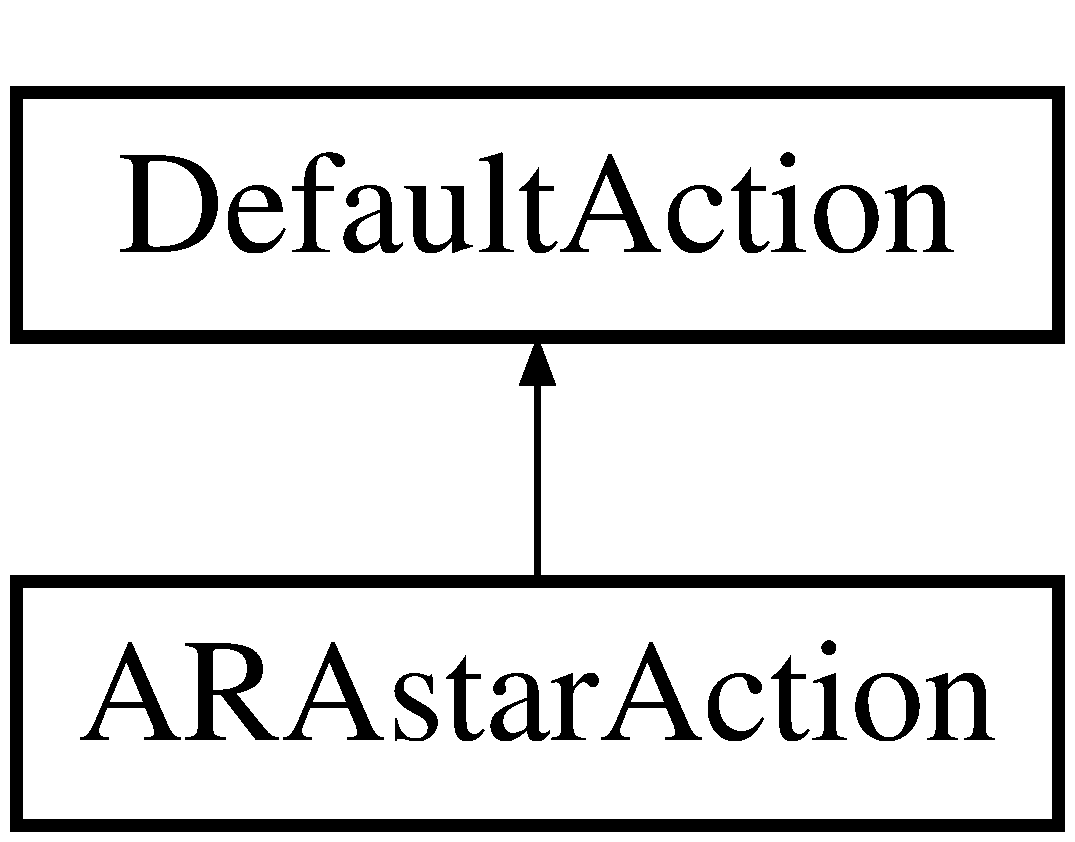
\includegraphics[height=2.000000cm]{class_a_r_astar_action}
\end{center}
\end{figure}
\subsection*{Public Member Functions}
\begin{DoxyCompactItemize}
\item 
\hyperlink{class_a_r_astar_action_a8df659204ab99fd85f1b925007cf17e7}{A\-R\-Astar\-Action} ()
\begin{DoxyCompactList}\small\item\em Initializes a new instance of the \hyperlink{class_a_r_astar_action}{A\-R\-Astar\-Action} class. \end{DoxyCompactList}\item 
\hyperlink{class_a_r_astar_action_a953c37f988df7b6c603c22e326b8180e}{A\-R\-Astar\-Action} (\hyperlink{class_default_state}{Default\-State} \-\_\-from, \hyperlink{class_default_state}{Default\-State} \-\_\-to)
\begin{DoxyCompactList}\small\item\em Initializes a new instance of the \hyperlink{class_a_r_astar_action}{A\-R\-Astar\-Action} class. \end{DoxyCompactList}\end{DoxyCompactItemize}
\subsection*{Public Attributes}
\begin{DoxyCompactItemize}
\item 
\hypertarget{class_a_r_astar_action_a67c203d535ee1b18ddec483a74b5923e}{Vector3 \hyperlink{class_a_r_astar_action_a67c203d535ee1b18ddec483a74b5923e}{direction}}\label{class_a_r_astar_action_a67c203d535ee1b18ddec483a74b5923e}

\begin{DoxyCompactList}\small\item\em direction of the action given as a Vector3 \end{DoxyCompactList}\end{DoxyCompactItemize}


\subsection{Detailed Description}
Defines action used in grid domain test 

\subsection{Constructor \& Destructor Documentation}
\hypertarget{class_a_r_astar_action_a8df659204ab99fd85f1b925007cf17e7}{\index{A\-R\-Astar\-Action@{A\-R\-Astar\-Action}!A\-R\-Astar\-Action@{A\-R\-Astar\-Action}}
\index{A\-R\-Astar\-Action@{A\-R\-Astar\-Action}!ARAstarAction@{A\-R\-Astar\-Action}}
\subsubsection[{A\-R\-Astar\-Action}]{\setlength{\rightskip}{0pt plus 5cm}A\-R\-Astar\-Action.\-A\-R\-Astar\-Action (
\begin{DoxyParamCaption}
{}
\end{DoxyParamCaption}
)}}\label{class_a_r_astar_action_a8df659204ab99fd85f1b925007cf17e7}


Initializes a new instance of the \hyperlink{class_a_r_astar_action}{A\-R\-Astar\-Action} class. 

\hypertarget{class_a_r_astar_action_a953c37f988df7b6c603c22e326b8180e}{\index{A\-R\-Astar\-Action@{A\-R\-Astar\-Action}!A\-R\-Astar\-Action@{A\-R\-Astar\-Action}}
\index{A\-R\-Astar\-Action@{A\-R\-Astar\-Action}!ARAstarAction@{A\-R\-Astar\-Action}}
\subsubsection[{A\-R\-Astar\-Action}]{\setlength{\rightskip}{0pt plus 5cm}A\-R\-Astar\-Action.\-A\-R\-Astar\-Action (
\begin{DoxyParamCaption}
\item[{{\bf Default\-State}}]{\-\_\-from, }
\item[{{\bf Default\-State}}]{\-\_\-to}
\end{DoxyParamCaption}
)}}\label{class_a_r_astar_action_a953c37f988df7b6c603c22e326b8180e}


Initializes a new instance of the \hyperlink{class_a_r_astar_action}{A\-R\-Astar\-Action} class. 


\begin{DoxyParams}{Parameters}
{\em \-\_\-from} & State where the transition is made from \\
\hline
{\em \-\_\-to} & State where the transition is made to \\
\hline
\end{DoxyParams}


The documentation for this class was generated from the following file\-:\begin{DoxyCompactItemize}
\item 
V\-A\-S\-T/vast/\-Assets/\-Plannar Scripts/\-Planners In Use/A\-R\-Astar\-Test.\-cs\end{DoxyCompactItemize}

\hypertarget{class_a_r_astar_domain}{\section{A\-R\-Astar\-Domain Class Reference}
\label{class_a_r_astar_domain}\index{A\-R\-Astar\-Domain@{A\-R\-Astar\-Domain}}
}
Inheritance diagram for A\-R\-Astar\-Domain\-:\begin{figure}[H]
\begin{center}
\leavevmode
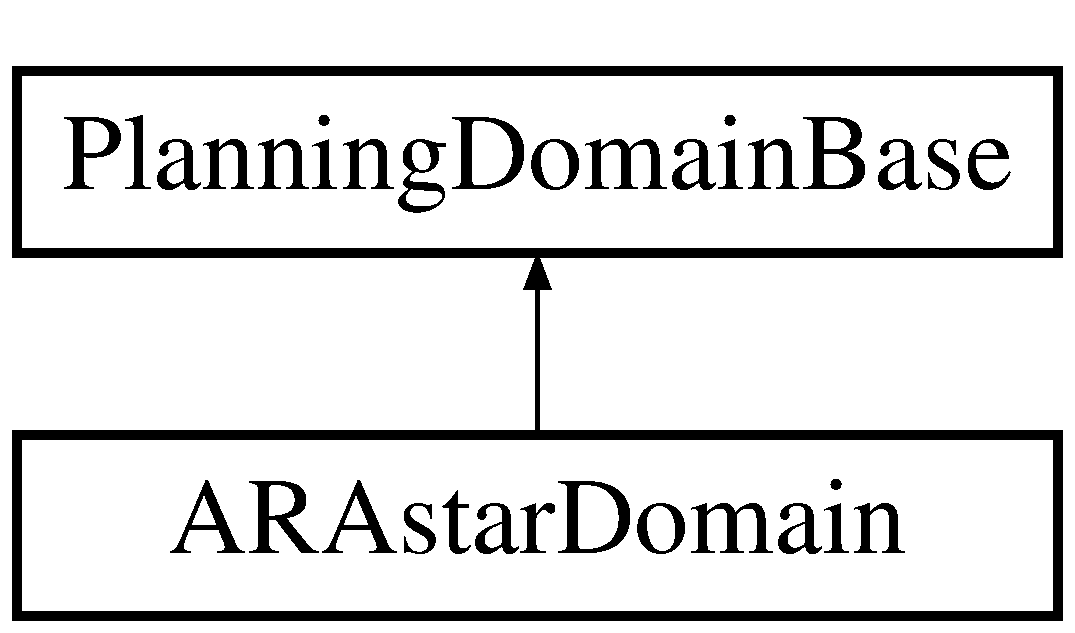
\includegraphics[height=2.000000cm]{class_a_r_astar_domain}
\end{center}
\end{figure}
\subsection*{Public Member Functions}
\begin{DoxyCompactItemize}
\item 
\hyperlink{class_a_r_astar_domain_a6bf71019a03f9d4f0fdfb7bca1b26f60}{A\-R\-Astar\-Domain} ()
\begin{DoxyCompactList}\small\item\em Initializes a new instance of the \hyperlink{class_a_r_astar_domain}{A\-R\-Astar\-Domain} class. \end{DoxyCompactList}\item 
\hypertarget{class_a_r_astar_domain_a4dc68e076d4738c797c22a52f7853fc3}{void {\bfseries set\-Planning\-Task} (Task t\-\_\-planning\-Task)}\label{class_a_r_astar_domain_a4dc68e076d4738c797c22a52f7853fc3}

\item 
override \hyperlink{class_default_action}{Default\-Action} \hyperlink{class_a_r_astar_domain_ab246607e9d2bcc02d129dc0414a4de33}{generate\-Action} (\hyperlink{class_default_state}{Default\-State} previous\-State, \hyperlink{class_default_state}{Default\-State} next\-State)
\begin{DoxyCompactList}\small\item\em Generates a new action. \end{DoxyCompactList}\item 
\hypertarget{class_a_r_astar_domain_a84137b03c38d5085c79ce15d42b8fa21}{override void {\bfseries clear\-At\-Beginning\-Of\-Every\-Plan\-Iteration} ()}\label{class_a_r_astar_domain_a84137b03c38d5085c79ce15d42b8fa21}

\item 
override bool \hyperlink{class_a_r_astar_domain_a98710baa163975101bee4a3b5c8ba439}{is\-A\-Goal\-State} (ref \hyperlink{class_default_state}{Default\-State} state, ref \hyperlink{class_default_state}{Default\-State} ideal\-Goal\-State)
\begin{DoxyCompactList}\small\item\em Determines whether the given state is a goal or not. \end{DoxyCompactList}\item 
\hypertarget{class_a_r_astar_domain_ae4a5180a514904b4e689da12746f1412}{override float {\bfseries evaluate\-Domain} (ref \hyperlink{class_default_state}{Default\-State} state)}\label{class_a_r_astar_domain_ae4a5180a514904b4e689da12746f1412}

\item 
override float \hyperlink{class_a_r_astar_domain_a94b2a2fb1766938d4da597ebf3fa16fd}{Compute\-H\-Estimate} (\hyperlink{class_default_state}{Default\-State} \-\_\-from, \hyperlink{class_default_state}{Default\-State} \-\_\-to)
\begin{DoxyCompactList}\small\item\em Computes the H estimate. \end{DoxyCompactList}\item 
override float \hyperlink{class_a_r_astar_domain_ae5d72a77811f6c7ec9eb48e2c4d895f0}{Compute\-G\-Estimate} (\hyperlink{class_default_state}{Default\-State} \-\_\-from, \hyperlink{class_default_state}{Default\-State} \-\_\-to)
\begin{DoxyCompactList}\small\item\em Computes the G estimate. \end{DoxyCompactList}\item 
override bool \hyperlink{class_a_r_astar_domain_a3da7327f8e5bf0594ba9ddb5c183475c}{equals} (\hyperlink{class_default_state}{Default\-State} s1, \hyperlink{class_default_state}{Default\-State} s2, bool is\-Start)
\begin{DoxyCompactList}\small\item\em Determines whether s1 is equals to s2. \end{DoxyCompactList}\item 
override void \hyperlink{class_a_r_astar_domain_a9d17ca7a84828a5af57ae2d8df034354}{generate\-Predecessors} (\hyperlink{class_default_state}{Default\-State} current\-State, ref List$<$ \hyperlink{class_default_action}{Default\-Action} $>$ action\-List)
\begin{DoxyCompactList}\small\item\em Generates the predecessors. \end{DoxyCompactList}\item 
override void \hyperlink{class_a_r_astar_domain_a16890b0a0fea5a007b3ad3264c39dd91}{generate\-Transitions} (ref \hyperlink{class_default_state}{Default\-State} current\-State, ref \hyperlink{class_default_state}{Default\-State} previous\-State, ref \hyperlink{class_default_state}{Default\-State} ideal\-Goal\-State, ref List$<$ \hyperlink{class_default_action}{Default\-Action} $>$ transitions)
\begin{DoxyCompactList}\small\item\em Generates possible transitions. \end{DoxyCompactList}\end{DoxyCompactItemize}
\subsection*{Additional Inherited Members}


\subsection{Detailed Description}
Defines domain used in grid domain test 

\subsection{Constructor \& Destructor Documentation}
\hypertarget{class_a_r_astar_domain_a6bf71019a03f9d4f0fdfb7bca1b26f60}{\index{A\-R\-Astar\-Domain@{A\-R\-Astar\-Domain}!A\-R\-Astar\-Domain@{A\-R\-Astar\-Domain}}
\index{A\-R\-Astar\-Domain@{A\-R\-Astar\-Domain}!ARAstarDomain@{A\-R\-Astar\-Domain}}
\subsubsection[{A\-R\-Astar\-Domain}]{\setlength{\rightskip}{0pt plus 5cm}A\-R\-Astar\-Domain.\-A\-R\-Astar\-Domain (
\begin{DoxyParamCaption}
{}
\end{DoxyParamCaption}
)}}\label{class_a_r_astar_domain_a6bf71019a03f9d4f0fdfb7bca1b26f60}


Initializes a new instance of the \hyperlink{class_a_r_astar_domain}{A\-R\-Astar\-Domain} class. 



\subsection{Member Function Documentation}
\hypertarget{class_a_r_astar_domain_ae5d72a77811f6c7ec9eb48e2c4d895f0}{\index{A\-R\-Astar\-Domain@{A\-R\-Astar\-Domain}!Compute\-G\-Estimate@{Compute\-G\-Estimate}}
\index{Compute\-G\-Estimate@{Compute\-G\-Estimate}!ARAstarDomain@{A\-R\-Astar\-Domain}}
\subsubsection[{Compute\-G\-Estimate}]{\setlength{\rightskip}{0pt plus 5cm}override float A\-R\-Astar\-Domain.\-Compute\-G\-Estimate (
\begin{DoxyParamCaption}
\item[{{\bf Default\-State}}]{\-\_\-from, }
\item[{{\bf Default\-State}}]{\-\_\-to}
\end{DoxyParamCaption}
)\hspace{0.3cm}{\ttfamily [virtual]}}}\label{class_a_r_astar_domain_ae5d72a77811f6c7ec9eb48e2c4d895f0}


Computes the G estimate. 

\begin{DoxyReturn}{Returns}
The G estimate value. 
\end{DoxyReturn}

\begin{DoxyParams}{Parameters}
{\em \-\_\-from} & The node for which we are trying to obtain the g estimate. \\
\hline
{\em \-\_\-to} & The node to which we are trying to obtain the cost. \\
\hline
\end{DoxyParams}


Reimplemented from \hyperlink{class_planning_domain_base}{Planning\-Domain\-Base}.

\hypertarget{class_a_r_astar_domain_a94b2a2fb1766938d4da597ebf3fa16fd}{\index{A\-R\-Astar\-Domain@{A\-R\-Astar\-Domain}!Compute\-H\-Estimate@{Compute\-H\-Estimate}}
\index{Compute\-H\-Estimate@{Compute\-H\-Estimate}!ARAstarDomain@{A\-R\-Astar\-Domain}}
\subsubsection[{Compute\-H\-Estimate}]{\setlength{\rightskip}{0pt plus 5cm}override float A\-R\-Astar\-Domain.\-Compute\-H\-Estimate (
\begin{DoxyParamCaption}
\item[{{\bf Default\-State}}]{\-\_\-from, }
\item[{{\bf Default\-State}}]{\-\_\-to}
\end{DoxyParamCaption}
)\hspace{0.3cm}{\ttfamily [virtual]}}}\label{class_a_r_astar_domain_a94b2a2fb1766938d4da597ebf3fa16fd}


Computes the H estimate. 

\begin{DoxyReturn}{Returns}
The H estimate value. 
\end{DoxyReturn}

\begin{DoxyParams}{Parameters}
{\em \-\_\-from} & The node for which we are trying to obtain the h estimate. \\
\hline
{\em \-\_\-to} & The goal node. \\
\hline
\end{DoxyParams}


Reimplemented from \hyperlink{class_planning_domain_base}{Planning\-Domain\-Base}.

\hypertarget{class_a_r_astar_domain_a3da7327f8e5bf0594ba9ddb5c183475c}{\index{A\-R\-Astar\-Domain@{A\-R\-Astar\-Domain}!equals@{equals}}
\index{equals@{equals}!ARAstarDomain@{A\-R\-Astar\-Domain}}
\subsubsection[{equals}]{\setlength{\rightskip}{0pt plus 5cm}override bool A\-R\-Astar\-Domain.\-equals (
\begin{DoxyParamCaption}
\item[{{\bf Default\-State}}]{s1, }
\item[{{\bf Default\-State}}]{s2, }
\item[{bool}]{is\-Start}
\end{DoxyParamCaption}
)\hspace{0.3cm}{\ttfamily [virtual]}}}\label{class_a_r_astar_domain_a3da7327f8e5bf0594ba9ddb5c183475c}


Determines whether s1 is equals to s2. 


\begin{DoxyParams}{Parameters}
{\em s1} & State 1 \\
\hline
{\em s2} & State 2 \\
\hline
{\em is\-Start} & is\-Start is a flag that could be used in case comparing start and goal use different thresholds. \\
\hline
\end{DoxyParams}


Reimplemented from \hyperlink{class_planning_domain_base}{Planning\-Domain\-Base}.

\hypertarget{class_a_r_astar_domain_ab246607e9d2bcc02d129dc0414a4de33}{\index{A\-R\-Astar\-Domain@{A\-R\-Astar\-Domain}!generate\-Action@{generate\-Action}}
\index{generate\-Action@{generate\-Action}!ARAstarDomain@{A\-R\-Astar\-Domain}}
\subsubsection[{generate\-Action}]{\setlength{\rightskip}{0pt plus 5cm}override {\bf Default\-Action} A\-R\-Astar\-Domain.\-generate\-Action (
\begin{DoxyParamCaption}
\item[{{\bf Default\-State}}]{previous\-State, }
\item[{{\bf Default\-State}}]{next\-State}
\end{DoxyParamCaption}
)\hspace{0.3cm}{\ttfamily [virtual]}}}\label{class_a_r_astar_domain_ab246607e9d2bcc02d129dc0414a4de33}


Generates a new action. 

\begin{DoxyReturn}{Returns}
Action generated. 
\end{DoxyReturn}

\begin{DoxyParams}{Parameters}
{\em previous\-State} & State where the action is being generated from. \\
\hline
{\em next\-State} & State where the action is being generated to. \\
\hline
\end{DoxyParams}


Reimplemented from \hyperlink{class_planning_domain_base}{Planning\-Domain\-Base}.

\hypertarget{class_a_r_astar_domain_a9d17ca7a84828a5af57ae2d8df034354}{\index{A\-R\-Astar\-Domain@{A\-R\-Astar\-Domain}!generate\-Predecessors@{generate\-Predecessors}}
\index{generate\-Predecessors@{generate\-Predecessors}!ARAstarDomain@{A\-R\-Astar\-Domain}}
\subsubsection[{generate\-Predecessors}]{\setlength{\rightskip}{0pt plus 5cm}override void A\-R\-Astar\-Domain.\-generate\-Predecessors (
\begin{DoxyParamCaption}
\item[{{\bf Default\-State}}]{current\-State, }
\item[{ref List$<$ {\bf Default\-Action} $>$}]{action\-List}
\end{DoxyParamCaption}
)\hspace{0.3cm}{\ttfamily [virtual]}}}\label{class_a_r_astar_domain_a9d17ca7a84828a5af57ae2d8df034354}


Generates the predecessors. 


\begin{DoxyParams}{Parameters}
{\em current\-State} & Current state. \\
\hline
{\em action\-List} & List that will contain all allowed actions to generate predecessors. \\
\hline
\end{DoxyParams}


Reimplemented from \hyperlink{class_planning_domain_base}{Planning\-Domain\-Base}.

\hypertarget{class_a_r_astar_domain_a16890b0a0fea5a007b3ad3264c39dd91}{\index{A\-R\-Astar\-Domain@{A\-R\-Astar\-Domain}!generate\-Transitions@{generate\-Transitions}}
\index{generate\-Transitions@{generate\-Transitions}!ARAstarDomain@{A\-R\-Astar\-Domain}}
\subsubsection[{generate\-Transitions}]{\setlength{\rightskip}{0pt plus 5cm}override void A\-R\-Astar\-Domain.\-generate\-Transitions (
\begin{DoxyParamCaption}
\item[{ref {\bf Default\-State}}]{current\-State, }
\item[{ref {\bf Default\-State}}]{previous\-State, }
\item[{ref {\bf Default\-State}}]{ideal\-Goal\-State, }
\item[{ref List$<$ {\bf Default\-Action} $>$}]{transitions}
\end{DoxyParamCaption}
)\hspace{0.3cm}{\ttfamily [virtual]}}}\label{class_a_r_astar_domain_a16890b0a0fea5a007b3ad3264c39dd91}


Generates possible transitions. 


\begin{DoxyParams}{Parameters}
{\em current\-State} & Current state. \\
\hline
{\em previous\-State} & Previous state. \\
\hline
{\em ideal\-Goal\-State} & Ideal goal state. \\
\hline
{\em transitions} & List that will contain all allowed transitions. \\
\hline
\end{DoxyParams}


Reimplemented from \hyperlink{class_planning_domain_base_adbca97ccf882076eb737b8bebf1fb1ea}{Planning\-Domain\-Base}.

\hypertarget{class_a_r_astar_domain_a98710baa163975101bee4a3b5c8ba439}{\index{A\-R\-Astar\-Domain@{A\-R\-Astar\-Domain}!is\-A\-Goal\-State@{is\-A\-Goal\-State}}
\index{is\-A\-Goal\-State@{is\-A\-Goal\-State}!ARAstarDomain@{A\-R\-Astar\-Domain}}
\subsubsection[{is\-A\-Goal\-State}]{\setlength{\rightskip}{0pt plus 5cm}override bool A\-R\-Astar\-Domain.\-is\-A\-Goal\-State (
\begin{DoxyParamCaption}
\item[{ref {\bf Default\-State}}]{state, }
\item[{ref {\bf Default\-State}}]{ideal\-Goal\-State}
\end{DoxyParamCaption}
)\hspace{0.3cm}{\ttfamily [virtual]}}}\label{class_a_r_astar_domain_a98710baa163975101bee4a3b5c8ba439}


Determines whether the given state is a goal or not. 

\begin{DoxyReturn}{Returns}
True if it is a goal and false otherwise. 
\end{DoxyReturn}

\begin{DoxyParams}{Parameters}
{\em state} & The state we are comparing to the goal \\
\hline
{\em ideal\-Goal\-State} & The goal staet we are trying to reach. \\
\hline
\end{DoxyParams}


Reimplemented from \hyperlink{class_planning_domain_base_a56907006c1e4a4071f58da65705792d1}{Planning\-Domain\-Base}.



The documentation for this class was generated from the following file\-:\begin{DoxyCompactItemize}
\item 
V\-A\-S\-T/vast/\-Assets/\-Plannar Scripts/\-Planners In Use/A\-R\-Astar\-Test.\-cs\end{DoxyCompactItemize}

\hypertarget{class_a_r_astar_heap}{\section{A\-R\-Astar\-Heap Class Reference}
\label{class_a_r_astar_heap}\index{A\-R\-Astar\-Heap@{A\-R\-Astar\-Heap}}
}
\subsection*{Public Member Functions}
\begin{DoxyCompactItemize}
\item 
\hypertarget{class_a_r_astar_heap_a699bf0a23b37f6f30ff2c04d2d445740}{{\bfseries A\-R\-Astar\-Heap} (float inflation\-Factor)}\label{class_a_r_astar_heap_a699bf0a23b37f6f30ff2c04d2d445740}

\item 
\hypertarget{class_a_r_astar_heap_aeb5fa05fb217b9650d2cd62b105b9a25}{\hyperlink{class_a_r_astar_node}{A\-R\-Astar\-Node} {\bfseries Heap\-Maximum} ()}\label{class_a_r_astar_heap_aeb5fa05fb217b9650d2cd62b105b9a25}

\item 
\hypertarget{class_a_r_astar_heap_a535db2f13d9af1e23757671601ad0f70}{\hyperlink{class_a_r_astar_node}{A\-R\-Astar\-Node} {\bfseries Extract\-Max} ()}\label{class_a_r_astar_heap_a535db2f13d9af1e23757671601ad0f70}

\item 
\hypertarget{class_a_r_astar_heap_a3ec8e0df935cb41937a202061caac700}{void {\bfseries Insert} (\hyperlink{class_a_r_astar_node}{A\-R\-Astar\-Node} node)}\label{class_a_r_astar_heap_a3ec8e0df935cb41937a202061caac700}

\item 
\hypertarget{class_a_r_astar_heap_a9ee6d644c983c0155159ee5ffa4d2801}{int {\bfseries Count} ()}\label{class_a_r_astar_heap_a9ee6d644c983c0155159ee5ffa4d2801}

\item 
\hypertarget{class_a_r_astar_heap_aae69fc99cd7df772bbfcfb6f3431c2ae}{void {\bfseries Remove} (\hyperlink{class_a_r_astar_node}{A\-R\-Astar\-Node} node)}\label{class_a_r_astar_heap_aae69fc99cd7df772bbfcfb6f3431c2ae}

\item 
\hypertarget{class_a_r_astar_heap_a700bc67c2fb4973bc75e3e9ad0fc4bca}{void {\bfseries Heapify} ()}\label{class_a_r_astar_heap_a700bc67c2fb4973bc75e3e9ad0fc4bca}

\end{DoxyCompactItemize}
\subsection*{Public Attributes}
\begin{DoxyCompactItemize}
\item 
\hypertarget{class_a_r_astar_heap_ae0f2f230149af325a9ee9865b0254a64}{List$<$ \hyperlink{class_a_r_astar_heap_node}{A\-R\-Astar\-Heap\-Node} $>$ {\bfseries heap}}\label{class_a_r_astar_heap_ae0f2f230149af325a9ee9865b0254a64}

\item 
\hypertarget{class_a_r_astar_heap_a2e92991656c5366efe99143fd372ee94}{float {\bfseries current\-Weight}}\label{class_a_r_astar_heap_a2e92991656c5366efe99143fd372ee94}

\end{DoxyCompactItemize}


The documentation for this class was generated from the following file\-:\begin{DoxyCompactItemize}
\item 
V\-A\-S\-T/vast/\-Assets/\-Plannar Scripts/\-Planners In Use/Heap.\-cs\end{DoxyCompactItemize}

\hypertarget{class_a_r_astar_heap_node}{\section{A\-R\-Astar\-Heap\-Node Class Reference}
\label{class_a_r_astar_heap_node}\index{A\-R\-Astar\-Heap\-Node@{A\-R\-Astar\-Heap\-Node}}
}
\subsection*{Public Member Functions}
\begin{DoxyCompactItemize}
\item 
\hypertarget{class_a_r_astar_heap_node_a024e3ef79561fc0c15a0f6420729e9b0}{{\bfseries A\-R\-Astar\-Heap\-Node} (\hyperlink{class_a_r_astar_node}{A\-R\-Astar\-Node} \-\_\-node, int \-\_\-index)}\label{class_a_r_astar_heap_node_a024e3ef79561fc0c15a0f6420729e9b0}

\end{DoxyCompactItemize}
\subsection*{Public Attributes}
\begin{DoxyCompactItemize}
\item 
\hypertarget{class_a_r_astar_heap_node_ac766db8d3cb63c58c56c73097ebb22d7}{\hyperlink{class_a_r_astar_node}{A\-R\-Astar\-Node} {\bfseries node}}\label{class_a_r_astar_heap_node_ac766db8d3cb63c58c56c73097ebb22d7}

\item 
\hypertarget{class_a_r_astar_heap_node_a3f8678a53e656f69e7aa5c5e2f35b59b}{int {\bfseries index}}\label{class_a_r_astar_heap_node_a3f8678a53e656f69e7aa5c5e2f35b59b}

\item 
\hypertarget{class_a_r_astar_heap_node_ab461374341ff031553fe8cd724410bf3}{int {\bfseries parent}}\label{class_a_r_astar_heap_node_ab461374341ff031553fe8cd724410bf3}

\item 
\hypertarget{class_a_r_astar_heap_node_a2dbbf8de61f62a3f548203fb5ad447b9}{int {\bfseries left\-Child}}\label{class_a_r_astar_heap_node_a2dbbf8de61f62a3f548203fb5ad447b9}

\item 
\hypertarget{class_a_r_astar_heap_node_a4722e1999dd6b0d3402796c82be44a44}{int {\bfseries right\-Child}}\label{class_a_r_astar_heap_node_a4722e1999dd6b0d3402796c82be44a44}

\end{DoxyCompactItemize}


The documentation for this class was generated from the following file\-:\begin{DoxyCompactItemize}
\item 
V\-A\-S\-T/vast/\-Assets/\-Plannar Scripts/\-Planners In Use/Heap.\-cs\end{DoxyCompactItemize}

\hypertarget{class_a_r_astar_node}{\section{A\-R\-Astar\-Node Class Reference}
\label{class_a_r_astar_node}\index{A\-R\-Astar\-Node@{A\-R\-Astar\-Node}}
}
\subsection*{Public Member Functions}
\begin{DoxyCompactItemize}
\item 
\hypertarget{class_a_r_astar_node_a9ab926f281a411131bce6855c7dffb8d}{\hyperlink{class_a_r_astar_node_a9ab926f281a411131bce6855c7dffb8d}{A\-R\-Astar\-Node} ()}\label{class_a_r_astar_node_a9ab926f281a411131bce6855c7dffb8d}

\begin{DoxyCompactList}\small\item\em Empty constructor. \end{DoxyCompactList}\item 
\hyperlink{class_a_r_astar_node_a248e2bfe43c8587087c91a9058cf1800}{A\-R\-Astar\-Node} (float \-\_\-g, float \-\_\-h, \hyperlink{class_default_state}{Default\-State} \-\_\-previous\-State\-Ref, \hyperlink{class_default_action}{Default\-Action} \-\_\-action\-Ref)
\begin{DoxyCompactList}\small\item\em Initializes a new instance of the \hyperlink{class_a_r_astar_node}{A\-R\-Astar\-Node} class. \end{DoxyCompactList}\item 
\hyperlink{class_a_r_astar_node_a99cdbb993be9eecbdd75614ce34f3131}{A\-R\-Astar\-Node} (float \-\_\-g, float \-\_\-h, \hyperlink{class_default_state}{Default\-State} \-\_\-previous\-State\-Ref, \hyperlink{class_default_state}{Default\-State} \-\_\-state\-Ref)
\begin{DoxyCompactList}\small\item\em Initializes a new instance of the \hyperlink{class_a_r_astar_node}{A\-R\-Astar\-Node} class. \end{DoxyCompactList}\item 
float\mbox{[}$\,$\mbox{]} \hyperlink{class_a_r_astar_node_ad270a3400cf18c3e937e9dd7e5d59c19}{Key} (float inflation\-Factor)
\begin{DoxyCompactList}\small\item\em Computes the given node's key. \end{DoxyCompactList}\end{DoxyCompactItemize}
\subsection*{Public Attributes}
\begin{DoxyCompactItemize}
\item 
\hypertarget{class_a_r_astar_node_ad8d5a3ba74c94fe21aafeb8b964c8a94}{float \hyperlink{class_a_r_astar_node_ad8d5a3ba74c94fe21aafeb8b964c8a94}{g}}\label{class_a_r_astar_node_ad8d5a3ba74c94fe21aafeb8b964c8a94}

\begin{DoxyCompactList}\small\item\em Node's g-\/value. \end{DoxyCompactList}\item 
\hypertarget{class_a_r_astar_node_aa9bc1b92b44c724c0b2c366fa9a37088}{float \hyperlink{class_a_r_astar_node_aa9bc1b92b44c724c0b2c366fa9a37088}{h}}\label{class_a_r_astar_node_aa9bc1b92b44c724c0b2c366fa9a37088}

\begin{DoxyCompactList}\small\item\em Node's h-\/value. \end{DoxyCompactList}\item 
\hypertarget{class_a_r_astar_node_a468f25ef194017b3c14eba82d6d35158}{float \hyperlink{class_a_r_astar_node_a468f25ef194017b3c14eba82d6d35158}{rhs}}\label{class_a_r_astar_node_a468f25ef194017b3c14eba82d6d35158}

\begin{DoxyCompactList}\small\item\em Node's one-\/step lookahead value. \end{DoxyCompactList}\item 
\hypertarget{class_a_r_astar_node_a653e0d399e1e9a7f4f970bb87fcaf257}{float \hyperlink{class_a_r_astar_node_a653e0d399e1e9a7f4f970bb87fcaf257}{weight\-Expanded} = 0}\label{class_a_r_astar_node_a653e0d399e1e9a7f4f970bb87fcaf257}

\begin{DoxyCompactList}\small\item\em Weight with which this node was created. \end{DoxyCompactList}\item 
\hypertarget{class_a_r_astar_node_ad3d169703b521311929565674575bf0d}{bool \hyperlink{class_a_r_astar_node_ad3d169703b521311929565674575bf0d}{is\-Dirty} = false}\label{class_a_r_astar_node_ad3d169703b521311929565674575bf0d}

\begin{DoxyCompactList}\small\item\em Dirty flag. \end{DoxyCompactList}\item 
\hypertarget{class_a_r_astar_node_ad77944d7b8ba8a5ea378a97e9a499f01}{bool \hyperlink{class_a_r_astar_node_ad77944d7b8ba8a5ea378a97e9a499f01}{touched} = false}\label{class_a_r_astar_node_ad77944d7b8ba8a5ea378a97e9a499f01}

\begin{DoxyCompactList}\small\item\em Touch flag. \end{DoxyCompactList}\item 
\hypertarget{class_a_r_astar_node_a04c5f46f811642b3d1ae617ad5587a10}{bool \hyperlink{class_a_r_astar_node_a04c5f46f811642b3d1ae617ad5587a10}{updated} = false}\label{class_a_r_astar_node_a04c5f46f811642b3d1ae617ad5587a10}

\begin{DoxyCompactList}\small\item\em Updated flag. \end{DoxyCompactList}\item 
\hypertarget{class_a_r_astar_node_a5b12783d756a225d773ae224a09cfa86}{int \hyperlink{class_a_r_astar_node_a5b12783d756a225d773ae224a09cfa86}{high\-Priority} = 0}\label{class_a_r_astar_node_a5b12783d756a225d773ae224a09cfa86}

\begin{DoxyCompactList}\small\item\em High priority counter. \end{DoxyCompactList}\item 
\hypertarget{class_a_r_astar_node_a9e2207d73d5a7aae1d08116c9da0e219}{\hyperlink{class_default_state}{Default\-State} \hyperlink{class_a_r_astar_node_a9e2207d73d5a7aae1d08116c9da0e219}{previous\-State}}\label{class_a_r_astar_node_a9e2207d73d5a7aae1d08116c9da0e219}

\begin{DoxyCompactList}\small\item\em Node's parent state. \end{DoxyCompactList}\item 
\hypertarget{class_a_r_astar_node_aa5991da6b78bc9e6c707c4906bef7e44}{\hyperlink{class_default_action}{Default\-Action} \hyperlink{class_a_r_astar_node_aa5991da6b78bc9e6c707c4906bef7e44}{action}}\label{class_a_r_astar_node_aa5991da6b78bc9e6c707c4906bef7e44}

\begin{DoxyCompactList}\small\item\em Action taken to reach this node. \end{DoxyCompactList}\end{DoxyCompactItemize}


\subsection{Detailed Description}
A\-R\-Astar Node This class represents a given state reached from a particular state. Many nodes could be associated with the same state as long as their parents differ from each other. 

\subsection{Constructor \& Destructor Documentation}
\hypertarget{class_a_r_astar_node_a248e2bfe43c8587087c91a9058cf1800}{\index{A\-R\-Astar\-Node@{A\-R\-Astar\-Node}!A\-R\-Astar\-Node@{A\-R\-Astar\-Node}}
\index{A\-R\-Astar\-Node@{A\-R\-Astar\-Node}!ARAstarNode@{A\-R\-Astar\-Node}}
\subsubsection[{A\-R\-Astar\-Node}]{\setlength{\rightskip}{0pt plus 5cm}A\-R\-Astar\-Node.\-A\-R\-Astar\-Node (
\begin{DoxyParamCaption}
\item[{float}]{\-\_\-g, }
\item[{float}]{\-\_\-h, }
\item[{{\bf Default\-State}}]{\-\_\-previous\-State\-Ref, }
\item[{{\bf Default\-Action}}]{\-\_\-action\-Ref}
\end{DoxyParamCaption}
)}}\label{class_a_r_astar_node_a248e2bfe43c8587087c91a9058cf1800}


Initializes a new instance of the \hyperlink{class_a_r_astar_node}{A\-R\-Astar\-Node} class. 


\begin{DoxyParams}{Parameters}
{\em \-\_\-g} & Node g-\/value \\
\hline
{\em \-\_\-h} & Node h-\/value \\
\hline
{\em \-\_\-previous\-State\-Ref} & Node's parent's state \\
\hline
{\em \-\_\-action\-Ref} & Action taken to generate node \\
\hline
\end{DoxyParams}
\hypertarget{class_a_r_astar_node_a99cdbb993be9eecbdd75614ce34f3131}{\index{A\-R\-Astar\-Node@{A\-R\-Astar\-Node}!A\-R\-Astar\-Node@{A\-R\-Astar\-Node}}
\index{A\-R\-Astar\-Node@{A\-R\-Astar\-Node}!ARAstarNode@{A\-R\-Astar\-Node}}
\subsubsection[{A\-R\-Astar\-Node}]{\setlength{\rightskip}{0pt plus 5cm}A\-R\-Astar\-Node.\-A\-R\-Astar\-Node (
\begin{DoxyParamCaption}
\item[{float}]{\-\_\-g, }
\item[{float}]{\-\_\-h, }
\item[{{\bf Default\-State}}]{\-\_\-previous\-State\-Ref, }
\item[{{\bf Default\-State}}]{\-\_\-state\-Ref}
\end{DoxyParamCaption}
)}}\label{class_a_r_astar_node_a99cdbb993be9eecbdd75614ce34f3131}


Initializes a new instance of the \hyperlink{class_a_r_astar_node}{A\-R\-Astar\-Node} class. 


\begin{DoxyParams}{Parameters}
{\em \-\_\-g} & Node's g-\/value \\
\hline
{\em \-\_\-h} & Node's h-\/value \\
\hline
{\em \-\_\-previous\-State\-Ref} & Node's parent's state \\
\hline
{\em \-\_\-state\-Ref} & Node's state \\
\hline
\end{DoxyParams}


\subsection{Member Function Documentation}
\hypertarget{class_a_r_astar_node_ad270a3400cf18c3e937e9dd7e5d59c19}{\index{A\-R\-Astar\-Node@{A\-R\-Astar\-Node}!Key@{Key}}
\index{Key@{Key}!ARAstarNode@{A\-R\-Astar\-Node}}
\subsubsection[{Key}]{\setlength{\rightskip}{0pt plus 5cm}float \mbox{[}$\,$\mbox{]} A\-R\-Astar\-Node.\-Key (
\begin{DoxyParamCaption}
\item[{float}]{inflation\-Factor}
\end{DoxyParamCaption}
)}}\label{class_a_r_astar_node_ad270a3400cf18c3e937e9dd7e5d59c19}


Computes the given node's key. 


\begin{DoxyParams}{Parameters}
{\em inflation\-Factor} & \hyperlink{class_planner}{Planner}'s current inflation factor \\
\hline
\end{DoxyParams}


The documentation for this class was generated from the following file\-:\begin{DoxyCompactItemize}
\item 
V\-A\-S\-T/vast/\-Assets/\-Plannar Scripts/\-Planners In Use/A\-R\-Astar\-Node.\-cs\end{DoxyCompactItemize}

\hypertarget{class_a_r_astar_planner}{\section{A\-R\-Astar\-Planner Class Reference}
\label{class_a_r_astar_planner}\index{A\-R\-Astar\-Planner@{A\-R\-Astar\-Planner}}
}
\subsection*{Public Member Functions}
\begin{DoxyCompactItemize}
\item 
\hyperlink{class_a_r_astar_planner_ac104ddca5d41bcceef98695c684d6fd1}{A\-R\-Astar\-Planner} ()
\begin{DoxyCompactList}\small\item\em Initializes a new instance of the \hyperlink{class_a_r_astar_planner}{A\-R\-Astar\-Planner} class. \end{DoxyCompactList}\item 
void \hyperlink{class_a_r_astar_planner_adb738f472ed71c2ef472a4dcd5c4a5f9}{init} (ref List$<$ \hyperlink{class_planning_domain_base}{Planning\-Domain\-Base} $>$ new\-Planning\-Domain, int max\-Num\-Nodes\-To\-Expand)
\begin{DoxyCompactList}\small\item\em Initializes required data for the planner. \end{DoxyCompactList}\item 
void \hyperlink{class_a_r_astar_planner_a02a2eeca8d5662b6179d003d3b21be8c}{Perform\-One\-Step} ()
\begin{DoxyCompactList}\small\item\em Performs one step of the planner. \end{DoxyCompactList}\item 
Path\-Status \hyperlink{class_a_r_astar_planner_aef22ec1bfe13cad24e8c7f0f0eb526ba}{compute\-Plan} (ref \hyperlink{class_default_state}{Default\-State} current\-State, ref \hyperlink{class_default_state}{Default\-State} \-\_\-goal\-State, ref Dictionary$<$ \hyperlink{class_default_state}{Default\-State}, \hyperlink{class_a_r_astar_node}{A\-R\-Astar\-Node} $>$ plan, ref float inflation, float max\-Time)
\begin{DoxyCompactList}\small\item\em Computes the plan. \end{DoxyCompactList}\item 
\hyperlink{class_default_state}{Default\-State} \hyperlink{class_a_r_astar_planner_aa6fea4b120f0db2d5b23045279d51bb5}{Fill\-Plan} ()
\begin{DoxyCompactList}\small\item\em Fills the plan. \end{DoxyCompactList}\item 
float \hyperlink{class_a_r_astar_planner_a006ae9bee4b3f93f82e79d4e103553ad}{fvalue} (\hyperlink{class_a_r_astar_node}{A\-R\-Astar\-Node} node)
\begin{DoxyCompactList}\small\item\em Computes a node's f-\/value. \end{DoxyCompactList}\item 
\hypertarget{class_a_r_astar_planner_ad129d7fbfc86b727772647edcaa62bce}{bool {\bfseries \-\_\-compute\-Plan} (ref \hyperlink{class_default_state}{Default\-State} start\-State, ref \hyperlink{class_default_state}{Default\-State} ideal\-Goal\-State, Dictionary$<$ \hyperlink{class_default_state}{Default\-State}, \hyperlink{class_a_r_astar_node}{A\-R\-Astar\-Node} $>$ map, ref \hyperlink{class_default_state}{Default\-State} actual\-State\-Reached, float max\-Time)}\label{class_a_r_astar_planner_ad129d7fbfc86b727772647edcaa62bce}

\item 
void \hyperlink{class_a_r_astar_planner_a61d4f2f23e1515ef5a9eaa74924ac447}{Visualize\-Container} (Container\-Type container\-Type, Color color, float radius)
\begin{DoxyCompactList}\small\item\em Visualizes the containers for debugging. \end{DoxyCompactList}\item 
void \hyperlink{class_a_r_astar_planner_a11fccda58571dcb091da9babda39ebd6}{Update\-After\-Obstacle\-Moved} (\hyperlink{class_default_state}{Default\-State} prev\-Obstacle\-State, \hyperlink{class_default_state}{Default\-State} current\-Obstacle\-State)
\begin{DoxyCompactList}\small\item\em Perfmors necessary updates after obstacle moved. \end{DoxyCompactList}\item 
\hypertarget{class_a_r_astar_planner_afb83f1df56770d7eab8f26498d00b8b6}{void {\bfseries set\-Selected\-Domain} (\hyperlink{class_planning_domain_base}{Planning\-Domain\-Base} domain)}\label{class_a_r_astar_planner_afb83f1df56770d7eab8f26498d00b8b6}

\item 
void \hyperlink{class_a_r_astar_planner_aa5e93fed6680adb3a8e1c0d84b7a6bc1}{Update\-After\-Goal\-Moved} (\hyperlink{class_default_state}{Default\-State} current\-Goal\-State)
\begin{DoxyCompactList}\small\item\em Performs the necessary updates after the goal moved. \end{DoxyCompactList}\item 
void \hyperlink{class_a_r_astar_planner_a5cead1843fe3fce8f0a222fdb5ae0192}{Update\-After\-Start\-Moved} (\hyperlink{class_default_state}{Default\-State} current\-State)
\begin{DoxyCompactList}\small\item\em Performs the necessary updates after start moved. \end{DoxyCompactList}\end{DoxyCompactItemize}
\subsection*{Public Attributes}
\begin{DoxyCompactItemize}
\item 
\hypertarget{class_a_r_astar_planner_a093fb1dbafd57ec94a5103ddc1679fc4}{int \hyperlink{class_a_r_astar_planner_a093fb1dbafd57ec94a5103ddc1679fc4}{\-\_\-max\-Num\-Nodes\-To\-Expand}}\label{class_a_r_astar_planner_a093fb1dbafd57ec94a5103ddc1679fc4}

\begin{DoxyCompactList}\small\item\em Maximum number of nodes to expand in a plan iteration. \end{DoxyCompactList}\item 
\hypertarget{class_a_r_astar_planner_ab31142d8f16ef4866ff6932098642fb5}{bool \hyperlink{class_a_r_astar_planner_ab31142d8f16ef4866ff6932098642fb5}{using\-Heap} = true}\label{class_a_r_astar_planner_ab31142d8f16ef4866ff6932098642fb5}

\begin{DoxyCompactList}\small\item\em Flag to determine if we sort with a heap (testing) \end{DoxyCompactList}\item 
\hypertarget{class_a_r_astar_planner_aa8318cf3bb76371812d9fffc4f4d0e9a}{float \hyperlink{class_a_r_astar_planner_aa8318cf3bb76371812d9fffc4f4d0e9a}{inflation\-Factor} = 1.\-0f}\label{class_a_r_astar_planner_aa8318cf3bb76371812d9fffc4f4d0e9a}

\begin{DoxyCompactList}\small\item\em Weight applied to heuristic. \end{DoxyCompactList}\item 
\hypertarget{class_a_r_astar_planner_a6df1ebaf2825a698b4cdec8e31da53bd}{bool \hyperlink{class_a_r_astar_planner_a6df1ebaf2825a698b4cdec8e31da53bd}{first\-Time} = true}\label{class_a_r_astar_planner_a6df1ebaf2825a698b4cdec8e31da53bd}

\begin{DoxyCompactList}\small\item\em Flag to determine if it's the first iteration. \end{DoxyCompactList}\item 
\hypertarget{class_a_r_astar_planner_aaffc01fe24f512518ba8ec49a6900f8a}{bool \hyperlink{class_a_r_astar_planner_aaffc01fe24f512518ba8ec49a6900f8a}{One\-Step} = false}\label{class_a_r_astar_planner_aaffc01fe24f512518ba8ec49a6900f8a}

\begin{DoxyCompactList}\small\item\em Flag to determine if we run planner step by step. \end{DoxyCompactList}\item 
\hypertarget{class_a_r_astar_planner_ad9b64f26b9a88475f983c4eb493de054}{List$<$ \hyperlink{class_planning_domain_base}{Planning\-Domain\-Base} $>$ \hyperlink{class_a_r_astar_planner_ad9b64f26b9a88475f983c4eb493de054}{\-\_\-planning\-Domain}}\label{class_a_r_astar_planner_ad9b64f26b9a88475f983c4eb493de054}

\begin{DoxyCompactList}\small\item\em List of possible domains. \end{DoxyCompactList}\item 
\hypertarget{class_a_r_astar_planner_aee2b292cb501a1495c039524e1ad8e94}{Dictionary$<$ \hyperlink{class_default_state}{Default\-State}, \\*
\hyperlink{class_a_r_astar_node}{A\-R\-Astar\-Node} $>$ \hyperlink{class_a_r_astar_planner_aee2b292cb501a1495c039524e1ad8e94}{Visited}}\label{class_a_r_astar_planner_aee2b292cb501a1495c039524e1ad8e94}

\begin{DoxyCompactList}\small\item\em Nodes visited so far. \end{DoxyCompactList}\item 
\hypertarget{class_a_r_astar_planner_af023a548cb94909a1b2c0e51988502b5}{\hyperlink{class_close_container}{Close\-Container} \hyperlink{class_a_r_astar_planner_af023a548cb94909a1b2c0e51988502b5}{Close}}\label{class_a_r_astar_planner_af023a548cb94909a1b2c0e51988502b5}

\begin{DoxyCompactList}\small\item\em List of nodes expanded. \end{DoxyCompactList}\item 
\hypertarget{class_a_r_astar_planner_ad5c4d105b353c64c6f0eab3d543d68dc}{\hyperlink{class_open_container}{Open\-Container} \hyperlink{class_a_r_astar_planner_ad5c4d105b353c64c6f0eab3d543d68dc}{Open}}\label{class_a_r_astar_planner_ad5c4d105b353c64c6f0eab3d543d68dc}

\begin{DoxyCompactList}\small\item\em List of nodes to expand. \end{DoxyCompactList}\item 
\hypertarget{class_a_r_astar_planner_ab01b3701ca3e0de21ee17603597e14e9}{\hyperlink{class_incons}{Incons} \hyperlink{class_a_r_astar_planner_ab01b3701ca3e0de21ee17603597e14e9}{Incons}}\label{class_a_r_astar_planner_ab01b3701ca3e0de21ee17603597e14e9}

\begin{DoxyCompactList}\small\item\em List of inconsistent nodes. \end{DoxyCompactList}\item 
\hypertarget{class_a_r_astar_planner_a94ca878be05551532a686abeb4a1d66e}{bool {\bfseries planner\-Finished} = false}\label{class_a_r_astar_planner_a94ca878be05551532a686abeb4a1d66e}

\end{DoxyCompactItemize}
\subsection*{Static Public Attributes}
\begin{DoxyCompactItemize}
\item 
\hypertarget{class_a_r_astar_planner_a1e8434cfc5c8f0f3e6bd09e585296439}{static bool \hyperlink{class_a_r_astar_planner_a1e8434cfc5c8f0f3e6bd09e585296439}{moved} = false}\label{class_a_r_astar_planner_a1e8434cfc5c8f0f3e6bd09e585296439}

\begin{DoxyCompactList}\small\item\em Flag to determine if agent moved. \end{DoxyCompactList}\item 
\hypertarget{class_a_r_astar_planner_aee85a0fdc5f048dfee9cd3c58e2a6c35}{static bool \hyperlink{class_a_r_astar_planner_aee85a0fdc5f048dfee9cd3c58e2a6c35}{goal\-Moved} = false}\label{class_a_r_astar_planner_aee85a0fdc5f048dfee9cd3c58e2a6c35}

\begin{DoxyCompactList}\small\item\em Flag to determine if goal moved. \end{DoxyCompactList}\item 
\hypertarget{class_a_r_astar_planner_acd32a5682197c310f1c4f3660c218eca}{static bool \hyperlink{class_a_r_astar_planner_acd32a5682197c310f1c4f3660c218eca}{obstacle\-Moved} = false}\label{class_a_r_astar_planner_acd32a5682197c310f1c4f3660c218eca}

\begin{DoxyCompactList}\small\item\em Flag to determine if obstacle moved. \end{DoxyCompactList}\end{DoxyCompactItemize}


\subsection{Detailed Description}
This is the main class for A\-R\-Astar \hyperlink{class_planner}{Planner} Handles all details related to the search. 

\subsection{Constructor \& Destructor Documentation}
\hypertarget{class_a_r_astar_planner_ac104ddca5d41bcceef98695c684d6fd1}{\index{A\-R\-Astar\-Planner@{A\-R\-Astar\-Planner}!A\-R\-Astar\-Planner@{A\-R\-Astar\-Planner}}
\index{A\-R\-Astar\-Planner@{A\-R\-Astar\-Planner}!ARAstarPlanner@{A\-R\-Astar\-Planner}}
\subsubsection[{A\-R\-Astar\-Planner}]{\setlength{\rightskip}{0pt plus 5cm}A\-R\-Astar\-Planner.\-A\-R\-Astar\-Planner (
\begin{DoxyParamCaption}
{}
\end{DoxyParamCaption}
)}}\label{class_a_r_astar_planner_ac104ddca5d41bcceef98695c684d6fd1}


Initializes a new instance of the \hyperlink{class_a_r_astar_planner}{A\-R\-Astar\-Planner} class. 



\subsection{Member Function Documentation}
\hypertarget{class_a_r_astar_planner_aef22ec1bfe13cad24e8c7f0f0eb526ba}{\index{A\-R\-Astar\-Planner@{A\-R\-Astar\-Planner}!compute\-Plan@{compute\-Plan}}
\index{compute\-Plan@{compute\-Plan}!ARAstarPlanner@{A\-R\-Astar\-Planner}}
\subsubsection[{compute\-Plan}]{\setlength{\rightskip}{0pt plus 5cm}Path\-Status A\-R\-Astar\-Planner.\-compute\-Plan (
\begin{DoxyParamCaption}
\item[{ref {\bf Default\-State}}]{current\-State, }
\item[{ref {\bf Default\-State}}]{\-\_\-goal\-State, }
\item[{ref Dictionary$<$ {\bf Default\-State}, {\bf A\-R\-Astar\-Node} $>$}]{plan, }
\item[{ref float}]{inflation, }
\item[{float}]{max\-Time}
\end{DoxyParamCaption}
)}}\label{class_a_r_astar_planner_aef22ec1bfe13cad24e8c7f0f0eb526ba}


Computes the plan. 

\begin{DoxyReturn}{Returns}
Plan status. 
\end{DoxyReturn}

\begin{DoxyParams}{Parameters}
{\em current\-State} & Agent state. \\
\hline
{\em \-\_\-goal\-State} & Goal state. \\
\hline
{\em plan} & Dictionary where plan will be stored. \\
\hline
{\em inflation} & Inflation factor. \\
\hline
{\em max\-Time} & Maximum alloted time. \\
\hline
\end{DoxyParams}
\hypertarget{class_a_r_astar_planner_aa6fea4b120f0db2d5b23045279d51bb5}{\index{A\-R\-Astar\-Planner@{A\-R\-Astar\-Planner}!Fill\-Plan@{Fill\-Plan}}
\index{Fill\-Plan@{Fill\-Plan}!ARAstarPlanner@{A\-R\-Astar\-Planner}}
\subsubsection[{Fill\-Plan}]{\setlength{\rightskip}{0pt plus 5cm}{\bf Default\-State} A\-R\-Astar\-Planner.\-Fill\-Plan (
\begin{DoxyParamCaption}
{}
\end{DoxyParamCaption}
)}}\label{class_a_r_astar_planner_aa6fea4b120f0db2d5b23045279d51bb5}


Fills the plan. 

\begin{DoxyReturn}{Returns}
Closest state reached. 
\end{DoxyReturn}
\hypertarget{class_a_r_astar_planner_a006ae9bee4b3f93f82e79d4e103553ad}{\index{A\-R\-Astar\-Planner@{A\-R\-Astar\-Planner}!fvalue@{fvalue}}
\index{fvalue@{fvalue}!ARAstarPlanner@{A\-R\-Astar\-Planner}}
\subsubsection[{fvalue}]{\setlength{\rightskip}{0pt plus 5cm}float A\-R\-Astar\-Planner.\-fvalue (
\begin{DoxyParamCaption}
\item[{{\bf A\-R\-Astar\-Node}}]{node}
\end{DoxyParamCaption}
)}}\label{class_a_r_astar_planner_a006ae9bee4b3f93f82e79d4e103553ad}


Computes a node's f-\/value. 


\begin{DoxyParams}{Parameters}
{\em node} & Node. \\
\hline
\end{DoxyParams}
\hypertarget{class_a_r_astar_planner_adb738f472ed71c2ef472a4dcd5c4a5f9}{\index{A\-R\-Astar\-Planner@{A\-R\-Astar\-Planner}!init@{init}}
\index{init@{init}!ARAstarPlanner@{A\-R\-Astar\-Planner}}
\subsubsection[{init}]{\setlength{\rightskip}{0pt plus 5cm}void A\-R\-Astar\-Planner.\-init (
\begin{DoxyParamCaption}
\item[{ref List$<$ {\bf Planning\-Domain\-Base} $>$}]{new\-Planning\-Domain, }
\item[{int}]{max\-Num\-Nodes\-To\-Expand}
\end{DoxyParamCaption}
)}}\label{class_a_r_astar_planner_adb738f472ed71c2ef472a4dcd5c4a5f9}


Initializes required data for the planner. 


\begin{DoxyParams}{Parameters}
{\em new\-Planning\-Domain} & List of domains to be used \\
\hline
{\em max\-Num\-Nodes\-To\-Expand} & Maximum number of nodes to expand. \\
\hline
\end{DoxyParams}
\hypertarget{class_a_r_astar_planner_a02a2eeca8d5662b6179d003d3b21be8c}{\index{A\-R\-Astar\-Planner@{A\-R\-Astar\-Planner}!Perform\-One\-Step@{Perform\-One\-Step}}
\index{Perform\-One\-Step@{Perform\-One\-Step}!ARAstarPlanner@{A\-R\-Astar\-Planner}}
\subsubsection[{Perform\-One\-Step}]{\setlength{\rightskip}{0pt plus 5cm}void A\-R\-Astar\-Planner.\-Perform\-One\-Step (
\begin{DoxyParamCaption}
{}
\end{DoxyParamCaption}
)}}\label{class_a_r_astar_planner_a02a2eeca8d5662b6179d003d3b21be8c}


Performs one step of the planner. 

\hypertarget{class_a_r_astar_planner_aa5e93fed6680adb3a8e1c0d84b7a6bc1}{\index{A\-R\-Astar\-Planner@{A\-R\-Astar\-Planner}!Update\-After\-Goal\-Moved@{Update\-After\-Goal\-Moved}}
\index{Update\-After\-Goal\-Moved@{Update\-After\-Goal\-Moved}!ARAstarPlanner@{A\-R\-Astar\-Planner}}
\subsubsection[{Update\-After\-Goal\-Moved}]{\setlength{\rightskip}{0pt plus 5cm}void A\-R\-Astar\-Planner.\-Update\-After\-Goal\-Moved (
\begin{DoxyParamCaption}
\item[{{\bf Default\-State}}]{current\-Goal\-State}
\end{DoxyParamCaption}
)}}\label{class_a_r_astar_planner_aa5e93fed6680adb3a8e1c0d84b7a6bc1}


Performs the necessary updates after the goal moved. 


\begin{DoxyParams}{Parameters}
{\em current\-Goal\-State} & Current goal state. \\
\hline
\end{DoxyParams}
\hypertarget{class_a_r_astar_planner_a11fccda58571dcb091da9babda39ebd6}{\index{A\-R\-Astar\-Planner@{A\-R\-Astar\-Planner}!Update\-After\-Obstacle\-Moved@{Update\-After\-Obstacle\-Moved}}
\index{Update\-After\-Obstacle\-Moved@{Update\-After\-Obstacle\-Moved}!ARAstarPlanner@{A\-R\-Astar\-Planner}}
\subsubsection[{Update\-After\-Obstacle\-Moved}]{\setlength{\rightskip}{0pt plus 5cm}void A\-R\-Astar\-Planner.\-Update\-After\-Obstacle\-Moved (
\begin{DoxyParamCaption}
\item[{{\bf Default\-State}}]{prev\-Obstacle\-State, }
\item[{{\bf Default\-State}}]{current\-Obstacle\-State}
\end{DoxyParamCaption}
)}}\label{class_a_r_astar_planner_a11fccda58571dcb091da9babda39ebd6}


Perfmors necessary updates after obstacle moved. 


\begin{DoxyParams}{Parameters}
{\em prev\-Obstacle\-State} & State were the obstacle was previously in. \\
\hline
{\em current\-Obstacle\-State} & State where the obstacle is currently in. \\
\hline
\end{DoxyParams}
\hypertarget{class_a_r_astar_planner_a5cead1843fe3fce8f0a222fdb5ae0192}{\index{A\-R\-Astar\-Planner@{A\-R\-Astar\-Planner}!Update\-After\-Start\-Moved@{Update\-After\-Start\-Moved}}
\index{Update\-After\-Start\-Moved@{Update\-After\-Start\-Moved}!ARAstarPlanner@{A\-R\-Astar\-Planner}}
\subsubsection[{Update\-After\-Start\-Moved}]{\setlength{\rightskip}{0pt plus 5cm}void A\-R\-Astar\-Planner.\-Update\-After\-Start\-Moved (
\begin{DoxyParamCaption}
\item[{{\bf Default\-State}}]{current\-State}
\end{DoxyParamCaption}
)}}\label{class_a_r_astar_planner_a5cead1843fe3fce8f0a222fdb5ae0192}


Performs the necessary updates after start moved. 


\begin{DoxyParams}{Parameters}
{\em current\-State} & Current state. \\
\hline
\end{DoxyParams}
\hypertarget{class_a_r_astar_planner_a61d4f2f23e1515ef5a9eaa74924ac447}{\index{A\-R\-Astar\-Planner@{A\-R\-Astar\-Planner}!Visualize\-Container@{Visualize\-Container}}
\index{Visualize\-Container@{Visualize\-Container}!ARAstarPlanner@{A\-R\-Astar\-Planner}}
\subsubsection[{Visualize\-Container}]{\setlength{\rightskip}{0pt plus 5cm}void A\-R\-Astar\-Planner.\-Visualize\-Container (
\begin{DoxyParamCaption}
\item[{Container\-Type}]{container\-Type, }
\item[{Color}]{color, }
\item[{float}]{radius}
\end{DoxyParamCaption}
)}}\label{class_a_r_astar_planner_a61d4f2f23e1515ef5a9eaa74924ac447}


Visualizes the containers for debugging. 


\begin{DoxyParams}{Parameters}
{\em container\-Type} & Container type. \\
\hline
{\em color} & Color used for visualization. \\
\hline
{\em radius} & Radius of sphere. \\
\hline
\end{DoxyParams}


The documentation for this class was generated from the following file\-:\begin{DoxyCompactItemize}
\item 
V\-A\-S\-T/vast/\-Assets/\-Plannar Scripts/\-Planners In Use/A\-R\-Astar\-Planner.\-cs\end{DoxyCompactItemize}

\hypertarget{class_a_r_astar_state}{\section{A\-R\-Astar\-State Class Reference}
\label{class_a_r_astar_state}\index{A\-R\-Astar\-State@{A\-R\-Astar\-State}}
}
Inheritance diagram for A\-R\-Astar\-State\-:\begin{figure}[H]
\begin{center}
\leavevmode
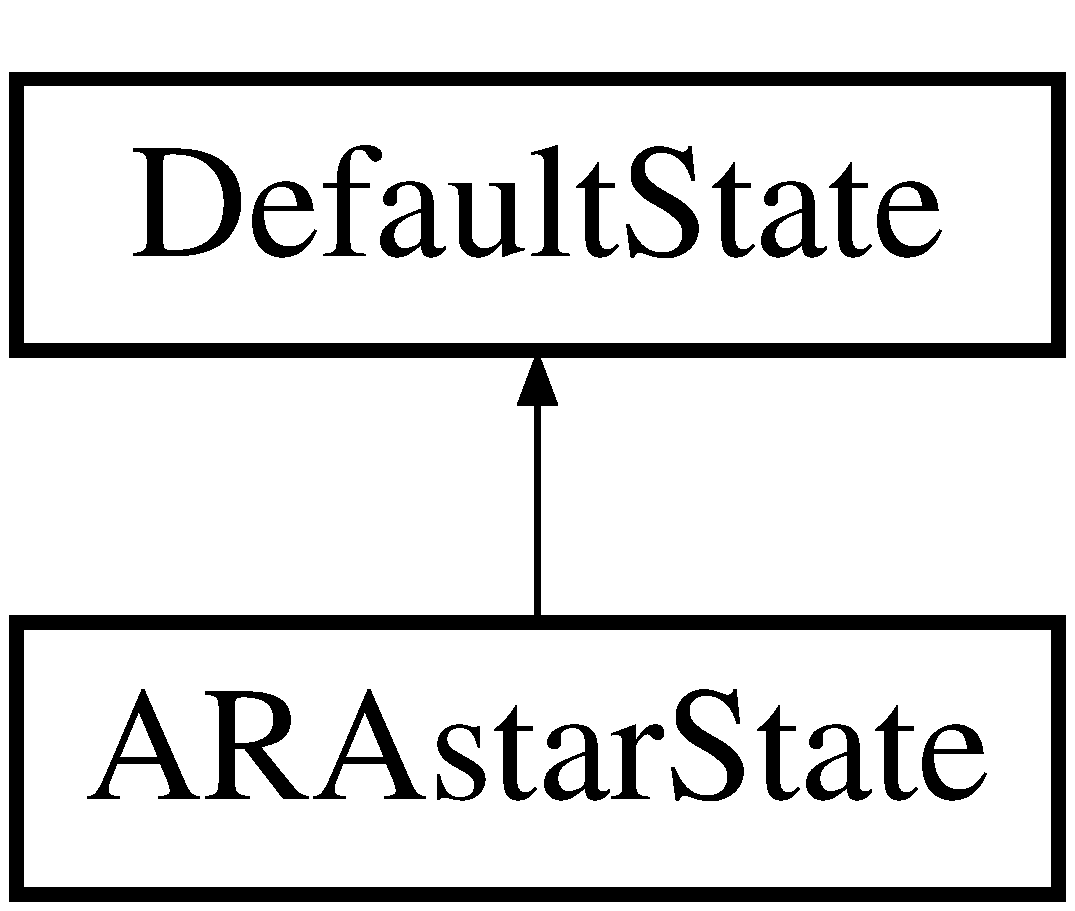
\includegraphics[height=2.000000cm]{class_a_r_astar_state}
\end{center}
\end{figure}
\subsection*{Public Member Functions}
\begin{DoxyCompactItemize}
\item 
\hypertarget{class_a_r_astar_state_aea1aef997b4a38111acaae49ca8b58e7}{{\bfseries A\-R\-Astar\-State} (Vector3 st)}\label{class_a_r_astar_state_aea1aef997b4a38111acaae49ca8b58e7}

\item 
\hypertarget{class_a_r_astar_state_a56f7f9692648f1824f7fbe8b5368c888}{override int {\bfseries Get\-Hash\-Code} ()}\label{class_a_r_astar_state_a56f7f9692648f1824f7fbe8b5368c888}

\item 
\hypertarget{class_a_r_astar_state_a09e066353969e553f2f1f6eaa3c3cd49}{override bool {\bfseries Equals} (object obj)}\label{class_a_r_astar_state_a09e066353969e553f2f1f6eaa3c3cd49}

\item 
\hypertarget{class_a_r_astar_state_ac382fe20a1cdfe2a2ce15cbd377c1c09}{bool {\bfseries Equals} (\hyperlink{class_a_r_astar_state}{A\-R\-Astar\-State} obj)}\label{class_a_r_astar_state_ac382fe20a1cdfe2a2ce15cbd377c1c09}

\item 
\hypertarget{class_a_r_astar_state_a0c13f3ba8101aae8654660f3fea953d5}{override Vector3 {\bfseries state\-Position} ()}\label{class_a_r_astar_state_a0c13f3ba8101aae8654660f3fea953d5}

\end{DoxyCompactItemize}
\subsection*{Public Attributes}
\begin{DoxyCompactItemize}
\item 
\hypertarget{class_a_r_astar_state_ae03c113a1d3d2e42ec3b4ee12a9c0ba8}{Vector3 {\bfseries state}}\label{class_a_r_astar_state_ae03c113a1d3d2e42ec3b4ee12a9c0ba8}

\end{DoxyCompactItemize}


\subsection{Detailed Description}
Defines state used in grid domain test 

The documentation for this class was generated from the following file\-:\begin{DoxyCompactItemize}
\item 
V\-A\-S\-T/vast/\-Assets/\-Plannar Scripts/\-Planners In Use/A\-R\-Astar\-Test.\-cs\end{DoxyCompactItemize}

\hypertarget{class_a_r_astar_test}{\section{A\-R\-Astar\-Test Class Reference}
\label{class_a_r_astar_test}\index{A\-R\-Astar\-Test@{A\-R\-Astar\-Test}}
}
\subsection*{Public Attributes}
\begin{DoxyCompactItemize}
\item 
\hypertarget{class_a_r_astar_test_a94aabd1964432001716ad2c0a8a2b86e}{Game\-Object {\bfseries start\-Object}}\label{class_a_r_astar_test_a94aabd1964432001716ad2c0a8a2b86e}

\item 
\hypertarget{class_a_r_astar_test_a58ab930498248f67873fabced04c3319}{bool {\bfseries using\-Heap}}\label{class_a_r_astar_test_a58ab930498248f67873fabced04c3319}

\item 
\hypertarget{class_a_r_astar_test_ac29fdf32984948271bfc5a96c1355d2b}{bool {\bfseries show\-Open}}\label{class_a_r_astar_test_ac29fdf32984948271bfc5a96c1355d2b}

\end{DoxyCompactItemize}
\subsection*{Static Public Attributes}
\begin{DoxyCompactItemize}
\item 
\hypertarget{class_a_r_astar_test_ae544bf76da132907014e8ec57c14167d}{static Dictionary\\*
$<$ \hyperlink{class_default_state}{Default\-State}, \hyperlink{class_a_r_astar_node}{A\-R\-Astar\-Node} $>$ {\bfseries output\-Plan}}\label{class_a_r_astar_test_ae544bf76da132907014e8ec57c14167d}

\end{DoxyCompactItemize}


\subsection{Detailed Description}
Grid domain test 

The documentation for this class was generated from the following file\-:\begin{DoxyCompactItemize}
\item 
V\-A\-S\-T/vast/\-Assets/\-Plannar Scripts/\-Planners In Use/A\-R\-Astar\-Test.\-cs\end{DoxyCompactItemize}

\hypertarget{class_best_first_action}{\section{Best\-First\-Action Class Reference}
\label{class_best_first_action}\index{Best\-First\-Action@{Best\-First\-Action}}
}
Inheritance diagram for Best\-First\-Action\-:\begin{figure}[H]
\begin{center}
\leavevmode
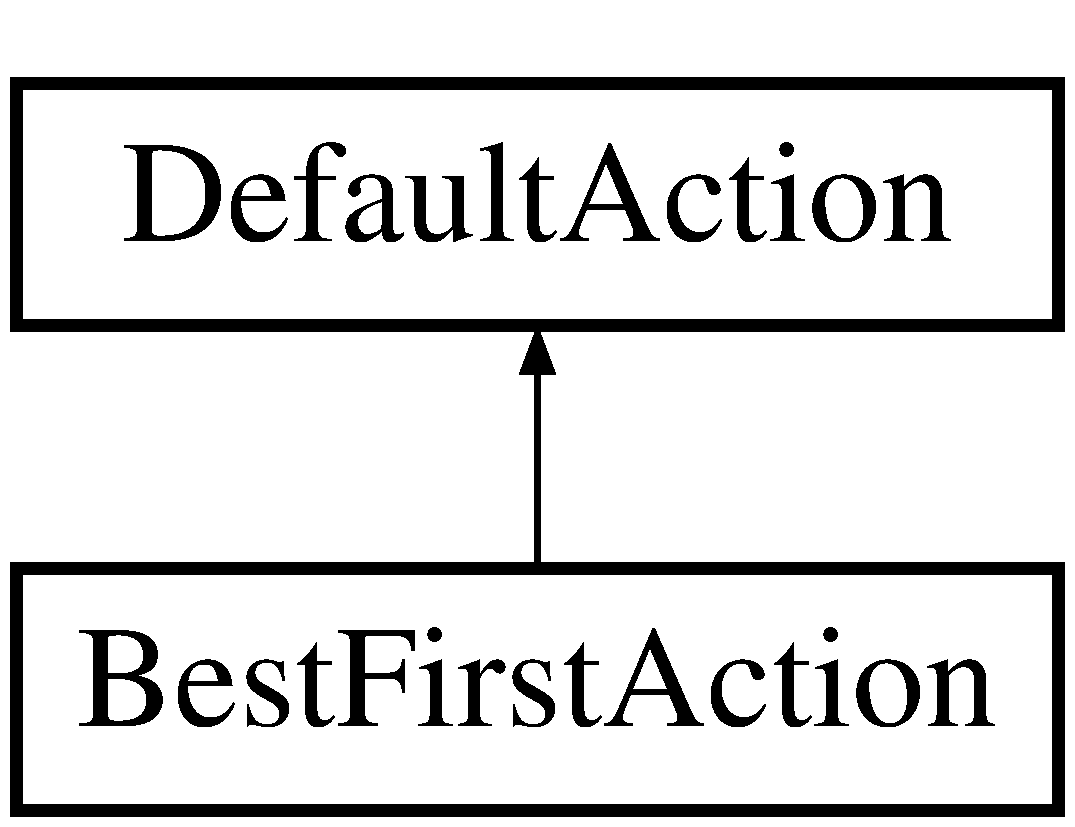
\includegraphics[height=2.000000cm]{class_best_first_action}
\end{center}
\end{figure}
\subsection*{Public Member Functions}
\begin{DoxyCompactItemize}
\item 
\hyperlink{class_best_first_action_ab9494d9bc38a672eb658f9026df0273a}{Best\-First\-Action} ()
\begin{DoxyCompactList}\small\item\em Initializes a new instance of the \hyperlink{class_best_first_action}{Best\-First\-Action} class. \end{DoxyCompactList}\item 
\hyperlink{class_best_first_action_a4bf1317d0be5523c3b6925fc2829ba4d}{Best\-First\-Action} (\hyperlink{class_default_state}{Default\-State} \-\_\-from, \hyperlink{class_default_state}{Default\-State} \-\_\-to)
\begin{DoxyCompactList}\small\item\em Initializes a new instance of the \hyperlink{class_best_first_action}{Best\-First\-Action} class. \end{DoxyCompactList}\end{DoxyCompactItemize}
\subsection*{Public Attributes}
\begin{DoxyCompactItemize}
\item 
\hypertarget{class_best_first_action_a20db99215323f8bb10f7bcbb90c5aa59}{Vector3 \hyperlink{class_best_first_action_a20db99215323f8bb10f7bcbb90c5aa59}{direction}}\label{class_best_first_action_a20db99215323f8bb10f7bcbb90c5aa59}

\begin{DoxyCompactList}\small\item\em The direction of the action as a Vector3. \end{DoxyCompactList}\end{DoxyCompactItemize}


\subsection{Detailed Description}
This class represents actions used in best first search planner. In this case it is a grid domain 

\subsection{Constructor \& Destructor Documentation}
\hypertarget{class_best_first_action_ab9494d9bc38a672eb658f9026df0273a}{\index{Best\-First\-Action@{Best\-First\-Action}!Best\-First\-Action@{Best\-First\-Action}}
\index{Best\-First\-Action@{Best\-First\-Action}!BestFirstAction@{Best\-First\-Action}}
\subsubsection[{Best\-First\-Action}]{\setlength{\rightskip}{0pt plus 5cm}Best\-First\-Action.\-Best\-First\-Action (
\begin{DoxyParamCaption}
{}
\end{DoxyParamCaption}
)}}\label{class_best_first_action_ab9494d9bc38a672eb658f9026df0273a}


Initializes a new instance of the \hyperlink{class_best_first_action}{Best\-First\-Action} class. 

\hypertarget{class_best_first_action_a4bf1317d0be5523c3b6925fc2829ba4d}{\index{Best\-First\-Action@{Best\-First\-Action}!Best\-First\-Action@{Best\-First\-Action}}
\index{Best\-First\-Action@{Best\-First\-Action}!BestFirstAction@{Best\-First\-Action}}
\subsubsection[{Best\-First\-Action}]{\setlength{\rightskip}{0pt plus 5cm}Best\-First\-Action.\-Best\-First\-Action (
\begin{DoxyParamCaption}
\item[{{\bf Default\-State}}]{\-\_\-from, }
\item[{{\bf Default\-State}}]{\-\_\-to}
\end{DoxyParamCaption}
)}}\label{class_best_first_action_a4bf1317d0be5523c3b6925fc2829ba4d}


Initializes a new instance of the \hyperlink{class_best_first_action}{Best\-First\-Action} class. 


\begin{DoxyParams}{Parameters}
{\em \-\_\-from} & The state this action is being taken from \\
\hline
{\em \-\_\-to} & The state this action leads to \\
\hline
\end{DoxyParams}


The documentation for this class was generated from the following file\-:\begin{DoxyCompactItemize}
\item 
V\-A\-S\-T/vast/\-Assets/\-Plannar Scripts/\-Planners In Use/Best\-First\-Search\-Test.\-cs\end{DoxyCompactItemize}

\hypertarget{class_best_first_domain}{\section{Best\-First\-Domain Class Reference}
\label{class_best_first_domain}\index{Best\-First\-Domain@{Best\-First\-Domain}}
}
Inheritance diagram for Best\-First\-Domain\-:\begin{figure}[H]
\begin{center}
\leavevmode
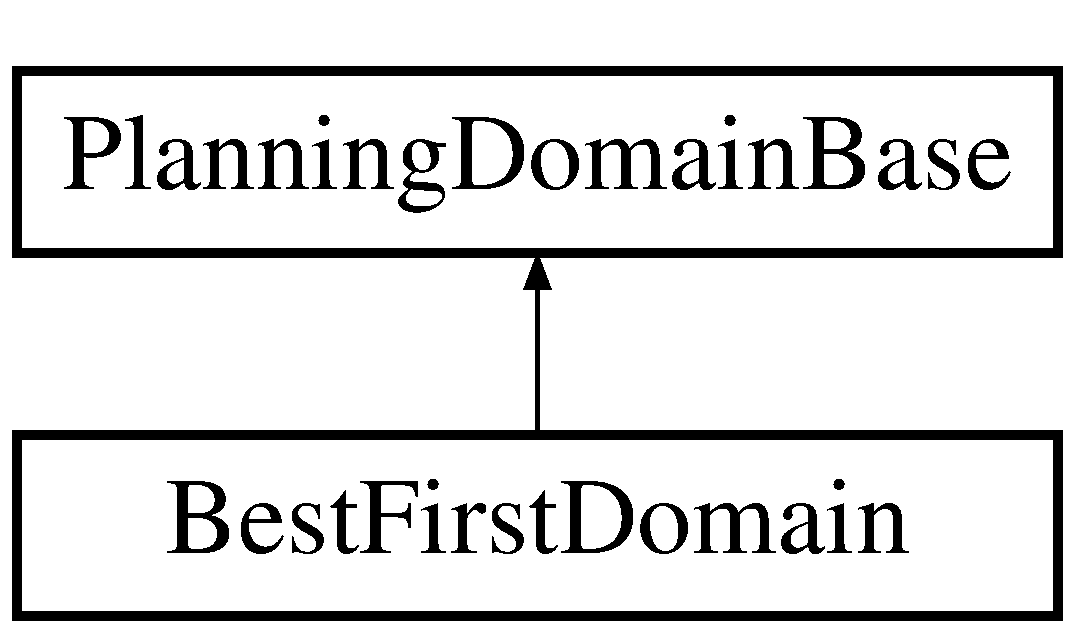
\includegraphics[height=2.000000cm]{class_best_first_domain}
\end{center}
\end{figure}
\subsection*{Public Member Functions}
\begin{DoxyCompactItemize}
\item 
\hypertarget{class_best_first_domain_a0b833b1832b075b88de09a79e277371b}{void {\bfseries set\-Planning\-Task} (Task t\-\_\-planning\-Task)}\label{class_best_first_domain_a0b833b1832b075b88de09a79e277371b}

\item 
\hypertarget{class_best_first_domain_a9b578aa834211cc398d3b1bbfb106752}{override \hyperlink{class_default_action}{Default\-Action} {\bfseries generate\-Action} (\hyperlink{class_default_state}{Default\-State} previous\-State, \hyperlink{class_default_state}{Default\-State} next\-State)}\label{class_best_first_domain_a9b578aa834211cc398d3b1bbfb106752}

\item 
override float \hyperlink{class_best_first_domain_a5e473a66ee8ebaec2674a63d06e6e278}{estimate\-Total\-Cost} (ref \hyperlink{class_default_state}{Default\-State} current\-State, ref \hyperlink{class_default_state}{Default\-State} ideal\-Goal\-State, float currentg)
\begin{DoxyCompactList}\small\item\em Computes the heuristic function (often denoted as f) that estimates the \char`\"{}goodness\char`\"{} of a state towards the goal. \end{DoxyCompactList}\item 
\hypertarget{class_best_first_domain_aadbbb1d21970c154374964f50b2a99d4}{override void {\bfseries clear\-At\-Beginning\-Of\-Every\-Plan\-Iteration} ()}\label{class_best_first_domain_aadbbb1d21970c154374964f50b2a99d4}

\item 
override bool \hyperlink{class_best_first_domain_a0f03bd6bd5617405d56f204732888d38}{is\-A\-Goal\-State} (ref \hyperlink{class_default_state}{Default\-State} state, ref \hyperlink{class_default_state}{Default\-State} ideal\-Goal\-State)
\begin{DoxyCompactList}\small\item\em Returns true if state is a valid goal state for the planning problem. \end{DoxyCompactList}\item 
\hypertarget{class_best_first_domain_a3b861f1177419c91174fa9b63b7d784b}{override float {\bfseries evaluate\-Domain} (ref \hyperlink{class_default_state}{Default\-State} state)}\label{class_best_first_domain_a3b861f1177419c91174fa9b63b7d784b}

\item 
\hypertarget{class_best_first_domain_a1d06e92291ef344534786f356393785d}{override float {\bfseries Compute\-H\-Estimate} (\hyperlink{class_default_state}{Default\-State} \-\_\-from, \hyperlink{class_default_state}{Default\-State} \-\_\-to)}\label{class_best_first_domain_a1d06e92291ef344534786f356393785d}

\item 
\hypertarget{class_best_first_domain_aa9143172a03294ce3ac98364281a761b}{override float {\bfseries Compute\-G\-Estimate} (\hyperlink{class_default_state}{Default\-State} \-\_\-from, \hyperlink{class_default_state}{Default\-State} \-\_\-to)}\label{class_best_first_domain_aa9143172a03294ce3ac98364281a761b}

\item 
\hypertarget{class_best_first_domain_ab7c02a966dfcd1c947e57dd96b27b86c}{override bool {\bfseries equals} (\hyperlink{class_default_state}{Default\-State} s1, \hyperlink{class_default_state}{Default\-State} s2, bool is\-Start)}\label{class_best_first_domain_ab7c02a966dfcd1c947e57dd96b27b86c}

\item 
\hypertarget{class_best_first_domain_ae63dbb2ad18a754752ddc8914a9c7f06}{override void {\bfseries generate\-Neighbors} (\hyperlink{class_default_state}{Default\-State} current\-State, ref List$<$ \hyperlink{class_default_state}{Default\-State} $>$ neighbors)}\label{class_best_first_domain_ae63dbb2ad18a754752ddc8914a9c7f06}

\item 
override void \hyperlink{class_best_first_domain_a06d5fdd90348af45d2f2de4944eacd6f}{generate\-Transitions} (ref \hyperlink{class_default_state}{Default\-State} current\-State, ref \hyperlink{class_default_state}{Default\-State} previous\-State, ref \hyperlink{class_default_state}{Default\-State} ideal\-Goal\-State, ref List$<$ \hyperlink{class_default_action}{Default\-Action} $>$ transitions)
\begin{DoxyCompactList}\small\item\em Populates the list of actions that can be taken from the current state. \end{DoxyCompactList}\end{DoxyCompactItemize}
\subsection*{Additional Inherited Members}


\subsection{Detailed Description}
Domain used in best first search planenr. This is a grid domain. 

\subsection{Member Function Documentation}
\hypertarget{class_best_first_domain_a5e473a66ee8ebaec2674a63d06e6e278}{\index{Best\-First\-Domain@{Best\-First\-Domain}!estimate\-Total\-Cost@{estimate\-Total\-Cost}}
\index{estimate\-Total\-Cost@{estimate\-Total\-Cost}!BestFirstDomain@{Best\-First\-Domain}}
\subsubsection[{estimate\-Total\-Cost}]{\setlength{\rightskip}{0pt plus 5cm}override float Best\-First\-Domain.\-estimate\-Total\-Cost (
\begin{DoxyParamCaption}
\item[{ref {\bf Default\-State}}]{current\-State, }
\item[{ref {\bf Default\-State}}]{ideal\-Goal\-State, }
\item[{float}]{currentg}
\end{DoxyParamCaption}
)\hspace{0.3cm}{\ttfamily [virtual]}}}\label{class_best_first_domain_a5e473a66ee8ebaec2674a63d06e6e278}


Computes the heuristic function (often denoted as f) that estimates the \char`\"{}goodness\char`\"{} of a state towards the goal. 

Note carerfully that this function should compute f, not h. For generalized best-\/first search, there is no explicit concept of h. For example, to implement A$\ast$, this function would return f, where f = currentg + h. In this case, h is the estimated distance or cost from the current state to the goal state. 

Reimplemented from \hyperlink{class_planning_domain_base_a4d0f803c0d3dfb3f59526078db674a4f}{Planning\-Domain\-Base}.

\hypertarget{class_best_first_domain_a06d5fdd90348af45d2f2de4944eacd6f}{\index{Best\-First\-Domain@{Best\-First\-Domain}!generate\-Transitions@{generate\-Transitions}}
\index{generate\-Transitions@{generate\-Transitions}!BestFirstDomain@{Best\-First\-Domain}}
\subsubsection[{generate\-Transitions}]{\setlength{\rightskip}{0pt plus 5cm}override void Best\-First\-Domain.\-generate\-Transitions (
\begin{DoxyParamCaption}
\item[{ref {\bf Default\-State}}]{current\-State, }
\item[{ref {\bf Default\-State}}]{previous\-State, }
\item[{ref {\bf Default\-State}}]{ideal\-Goal\-State, }
\item[{ref List$<$ {\bf Default\-Action} $>$}]{transitions}
\end{DoxyParamCaption}
)\hspace{0.3cm}{\ttfamily [virtual]}}}\label{class_best_first_domain_a06d5fdd90348af45d2f2de4944eacd6f}


Populates the list of actions that can be taken from the current state. 

When you implement this function, make sure that you initialize both the (1) cost and (2) new state of the action being generated.

You may wish to use the previous\-State or the ideal\-Goal\-State as additional information that helps you decide how to generate actions. The classic example of this is when the state space is a graph, you should avoid generating an action that will take you back to the previous graph node. In another example, you may choose to generate goal-\/dependent actions. 

Reimplemented from \hyperlink{class_planning_domain_base_adbca97ccf882076eb737b8bebf1fb1ea}{Planning\-Domain\-Base}.

\hypertarget{class_best_first_domain_a0f03bd6bd5617405d56f204732888d38}{\index{Best\-First\-Domain@{Best\-First\-Domain}!is\-A\-Goal\-State@{is\-A\-Goal\-State}}
\index{is\-A\-Goal\-State@{is\-A\-Goal\-State}!BestFirstDomain@{Best\-First\-Domain}}
\subsubsection[{is\-A\-Goal\-State}]{\setlength{\rightskip}{0pt plus 5cm}override bool Best\-First\-Domain.\-is\-A\-Goal\-State (
\begin{DoxyParamCaption}
\item[{ref {\bf Default\-State}}]{state, }
\item[{ref {\bf Default\-State}}]{ideal\-Goal\-State}
\end{DoxyParamCaption}
)\hspace{0.3cm}{\ttfamily [virtual]}}}\label{class_best_first_domain_a0f03bd6bd5617405d56f204732888d38}


Returns true if state is a valid goal state for the planning problem. 

The parameter ideal\-Goal\-State is only a reference to the goal state that the user specified when calling \hyperlink{class_best_first_search_planner_a777fb06939a33b3f3effb24b0dbda076}{Best\-First\-Search\-Planner\-::compute\-Plan()}. Depending on your planning task, you may want to ignore this value, for example, if you have multiple goals and only need to reach one of those goal states.

In most cases, however, this parameter is a helpful optimization, that allows you to compute \char`\"{}distance\char`\"{} or \char`\"{}cost\char`\"{} to the goal state without having to store extra data in your planning domain class. In some cases, this allows you to use the same instance of the planning domain for all agents that are performing the same planning task, even though they have different start and goal states. 

Reimplemented from \hyperlink{class_planning_domain_base_a56907006c1e4a4071f58da65705792d1}{Planning\-Domain\-Base}.



The documentation for this class was generated from the following file\-:\begin{DoxyCompactItemize}
\item 
V\-A\-S\-T/vast/\-Assets/\-Plannar Scripts/\-Planners In Use/Best\-First\-Search\-Test.\-cs\end{DoxyCompactItemize}

\hypertarget{class_best_first_search_node}{\section{Best\-First\-Search\-Node Class Reference}
\label{class_best_first_search_node}\index{Best\-First\-Search\-Node@{Best\-First\-Search\-Node}}
}


Internal helper class used to describe a node in the best-\/first search.  


\subsection*{Public Member Functions}
\begin{DoxyCompactItemize}
\item 
\hyperlink{class_best_first_search_node_acd51a5e054826ba7b3b56fadc77aed2e}{Best\-First\-Search\-Node} ()
\begin{DoxyCompactList}\small\item\em Initializes a new instance of the \hyperlink{class_best_first_search_node}{Best\-First\-Search\-Node} class. \end{DoxyCompactList}\item 
\hyperlink{class_best_first_search_node_afda8aef3a27e03d5d6252058970ea2f1}{Best\-First\-Search\-Node} (float \-\_\-g, float \-\_\-f, ref \hyperlink{class_default_state}{Default\-State} \-\_\-previous\-State\-Ref, ref \hyperlink{class_default_action}{Default\-Action} \-\_\-next\-Action\-Ref)
\begin{DoxyCompactList}\small\item\em Initializes a new instance of the \hyperlink{class_best_first_search_node}{Best\-First\-Search\-Node} class. \end{DoxyCompactList}\item 
\hyperlink{class_best_first_search_node_a4f3a23969ff7be7dcc574232dc2c6344}{Best\-First\-Search\-Node} (float \-\_\-g, float \-\_\-f, ref \hyperlink{class_default_state}{Default\-State} \-\_\-previous\-State\-Ref, ref \hyperlink{class_default_state}{Default\-State} \-\_\-next\-State\-Ref)
\begin{DoxyCompactList}\small\item\em Initializes a new instance of the \hyperlink{class_best_first_search_node}{Best\-First\-Search\-Node} class. \end{DoxyCompactList}\end{DoxyCompactItemize}
\subsection*{Public Attributes}
\begin{DoxyCompactItemize}
\item 
\hypertarget{class_best_first_search_node_ad6c65af451d6e2904c842833d49876c8}{float \hyperlink{class_best_first_search_node_ad6c65af451d6e2904c842833d49876c8}{g}}\label{class_best_first_search_node_ad6c65af451d6e2904c842833d49876c8}

\begin{DoxyCompactList}\small\item\em Node's g value. \end{DoxyCompactList}\item 
\hypertarget{class_best_first_search_node_a586a71b36b6621e0290f903c5b97adfd}{float \hyperlink{class_best_first_search_node_a586a71b36b6621e0290f903c5b97adfd}{f}}\label{class_best_first_search_node_a586a71b36b6621e0290f903c5b97adfd}

\begin{DoxyCompactList}\small\item\em Node's f value. \end{DoxyCompactList}\item 
\hypertarget{class_best_first_search_node_a9019b1e6f7cb4783ffb318cd58f726f4}{\hyperlink{class_default_state}{Default\-State} \hyperlink{class_best_first_search_node_a9019b1e6f7cb4783ffb318cd58f726f4}{previous\-State}}\label{class_best_first_search_node_a9019b1e6f7cb4783ffb318cd58f726f4}

\begin{DoxyCompactList}\small\item\em Node's parent state. \end{DoxyCompactList}\item 
\hypertarget{class_best_first_search_node_a8ec9adf5c8c0345a67f99e552da8e4e8}{\hyperlink{class_default_action}{Default\-Action} \hyperlink{class_best_first_search_node_a8ec9adf5c8c0345a67f99e552da8e4e8}{action}}\label{class_best_first_search_node_a8ec9adf5c8c0345a67f99e552da8e4e8}

\begin{DoxyCompactList}\small\item\em Action that was taken to reach this node. \end{DoxyCompactList}\item 
\hypertarget{class_best_first_search_node_a27b1fe54e186d21b8cabf78c87cabe02}{bool \hyperlink{class_best_first_search_node_a27b1fe54e186d21b8cabf78c87cabe02}{already\-Expanded}}\label{class_best_first_search_node_a27b1fe54e186d21b8cabf78c87cabe02}

\begin{DoxyCompactList}\small\item\em Flag to determine if the node was already expanded. \end{DoxyCompactList}\end{DoxyCompactItemize}


\subsection{Detailed Description}
Internal helper class used to describe a node in the best-\/first search. 

\begin{DoxyVerb}    This class is not intended to be used directly.  Instead, use the BestFirstSearchPlanner that
    uses this class for internal representation.

    @see
      - Documentation of the BestFirstSearchPlanner class, which describes how states and actions are used.   
\end{DoxyVerb}
 This class represents nodes used in best first search. 

\subsection{Constructor \& Destructor Documentation}
\hypertarget{class_best_first_search_node_acd51a5e054826ba7b3b56fadc77aed2e}{\index{Best\-First\-Search\-Node@{Best\-First\-Search\-Node}!Best\-First\-Search\-Node@{Best\-First\-Search\-Node}}
\index{Best\-First\-Search\-Node@{Best\-First\-Search\-Node}!BestFirstSearchNode@{Best\-First\-Search\-Node}}
\subsubsection[{Best\-First\-Search\-Node}]{\setlength{\rightskip}{0pt plus 5cm}Best\-First\-Search\-Node.\-Best\-First\-Search\-Node (
\begin{DoxyParamCaption}
{}
\end{DoxyParamCaption}
)}}\label{class_best_first_search_node_acd51a5e054826ba7b3b56fadc77aed2e}


Initializes a new instance of the \hyperlink{class_best_first_search_node}{Best\-First\-Search\-Node} class. 

\hypertarget{class_best_first_search_node_afda8aef3a27e03d5d6252058970ea2f1}{\index{Best\-First\-Search\-Node@{Best\-First\-Search\-Node}!Best\-First\-Search\-Node@{Best\-First\-Search\-Node}}
\index{Best\-First\-Search\-Node@{Best\-First\-Search\-Node}!BestFirstSearchNode@{Best\-First\-Search\-Node}}
\subsubsection[{Best\-First\-Search\-Node}]{\setlength{\rightskip}{0pt plus 5cm}Best\-First\-Search\-Node.\-Best\-First\-Search\-Node (
\begin{DoxyParamCaption}
\item[{float}]{\-\_\-g, }
\item[{float}]{\-\_\-f, }
\item[{ref {\bf Default\-State}}]{\-\_\-previous\-State\-Ref, }
\item[{ref {\bf Default\-Action}}]{\-\_\-next\-Action\-Ref}
\end{DoxyParamCaption}
)}}\label{class_best_first_search_node_afda8aef3a27e03d5d6252058970ea2f1}


Initializes a new instance of the \hyperlink{class_best_first_search_node}{Best\-First\-Search\-Node} class. 


\begin{DoxyParams}{Parameters}
{\em \-\_\-g} & Node's g-\/value \\
\hline
{\em \-\_\-f} & Node's f-\/value \\
\hline
{\em \-\_\-previous\-State\-Ref} & Reference to the state that originated this node \\
\hline
{\em \-\_\-next\-Action\-Ref} & Reference to the action that was taken to create this node \\
\hline
\end{DoxyParams}
\hypertarget{class_best_first_search_node_a4f3a23969ff7be7dcc574232dc2c6344}{\index{Best\-First\-Search\-Node@{Best\-First\-Search\-Node}!Best\-First\-Search\-Node@{Best\-First\-Search\-Node}}
\index{Best\-First\-Search\-Node@{Best\-First\-Search\-Node}!BestFirstSearchNode@{Best\-First\-Search\-Node}}
\subsubsection[{Best\-First\-Search\-Node}]{\setlength{\rightskip}{0pt plus 5cm}Best\-First\-Search\-Node.\-Best\-First\-Search\-Node (
\begin{DoxyParamCaption}
\item[{float}]{\-\_\-g, }
\item[{float}]{\-\_\-f, }
\item[{ref {\bf Default\-State}}]{\-\_\-previous\-State\-Ref, }
\item[{ref {\bf Default\-State}}]{\-\_\-next\-State\-Ref}
\end{DoxyParamCaption}
)}}\label{class_best_first_search_node_a4f3a23969ff7be7dcc574232dc2c6344}


Initializes a new instance of the \hyperlink{class_best_first_search_node}{Best\-First\-Search\-Node} class. 


\begin{DoxyParams}{Parameters}
{\em \-\_\-g} & Node's g-\/value \\
\hline
{\em \-\_\-f} & Node's f-\/value \\
\hline
{\em \-\_\-previous\-State\-Ref} & Reference to the state that was expanded to reach this node \\
\hline
{\em \-\_\-next\-State\-Ref} & Reference to the state this node represents \\
\hline
\end{DoxyParams}


The documentation for this class was generated from the following file\-:\begin{DoxyCompactItemize}
\item 
V\-A\-S\-T/vast/\-Assets/\-Plannar Scripts/\-Planners In Use/Best\-First\-Search\-Planner.\-cs\end{DoxyCompactItemize}

\hypertarget{class_best_first_search_planner}{\section{Best\-First\-Search\-Planner Class Reference}
\label{class_best_first_search_planner}\index{Best\-First\-Search\-Planner@{Best\-First\-Search\-Planner}}
}


A state-\/space planning algorithm that uses a generalized best-\/first search.  


\subsection*{Public Member Functions}
\begin{DoxyCompactItemize}
\item 
\hyperlink{class_best_first_search_planner_a66ba1fc8fab38445fe31cfa5297606c4}{Best\-First\-Search\-Planner} ()
\begin{DoxyCompactList}\small\item\em Initializes a new instance of the \hyperlink{class_best_first_search_planner}{Best\-First\-Search\-Planner} class. \end{DoxyCompactList}\item 
\hypertarget{class_best_first_search_planner_a00c06f79faf00907ec4906086c37776f}{void \hyperlink{class_best_first_search_planner_a00c06f79faf00907ec4906086c37776f}{init} (ref List$<$ \hyperlink{class_planning_domain_base}{Planning\-Domain\-Base} $>$ new\-Planning\-Domain, int max\-Num\-Nodes\-To\-Expand)}\label{class_best_first_search_planner_a00c06f79faf00907ec4906086c37776f}

\begin{DoxyCompactList}\small\item\em Initializes the planner to use the specified instance of the planning domain, and sets the search horizon limit. \end{DoxyCompactList}\item 
bool \hyperlink{class_best_first_search_planner_ab9066bb695cb64fc787f747a4972d878}{\-\_\-compute\-Plan} (ref \hyperlink{class_default_state}{Default\-State} start\-State, ref \hyperlink{class_default_state}{Default\-State} ideal\-Goal\-State, Dictionary$<$ \hyperlink{class_default_state}{Default\-State}, \hyperlink{class_best_first_search_node}{Best\-First\-Search\-Node} $>$ state\-Map, ref \hyperlink{class_default_state}{Default\-State} actual\-State\-Reached, float max\-Time)
\begin{DoxyCompactList}\small\item\em \-\_\-computes the plan. \end{DoxyCompactList}\item 
\hypertarget{class_best_first_search_planner_a97dc3cad80e236bde9c7d9c44759c7ba}{bool {\bfseries \-\_\-compute\-One\-Step} (ref \hyperlink{class_default_state}{Default\-State} start\-State, ref \hyperlink{class_default_state}{Default\-State} ideal\-Goal\-State, Dictionary$<$ \hyperlink{class_default_state}{Default\-State}, \hyperlink{class_best_first_search_node}{Best\-First\-Search\-Node} $>$ state\-Map, ref \hyperlink{class_default_state}{Default\-State} actual\-State\-Reached, float max\-Time)}\label{class_best_first_search_planner_a97dc3cad80e236bde9c7d9c44759c7ba}

\item 
\hypertarget{class_best_first_search_planner_a777fb06939a33b3f3effb24b0dbda076}{bool \hyperlink{class_best_first_search_planner_a777fb06939a33b3f3effb24b0dbda076}{compute\-Plan} (ref \hyperlink{class_default_state}{Default\-State} start\-State, ref \hyperlink{class_default_state}{Default\-State} goal\-State, ref Stack$<$ \hyperlink{class_default_state}{Default\-State} $>$ plan, float max\-Time)}\label{class_best_first_search_planner_a777fb06939a33b3f3effb24b0dbda076}

\begin{DoxyCompactList}\small\item\em Computes a plan as a sequence of states; returns true if the planner could reach the goal, or false if the plan is only partial and could not reach the goal within the specified horizon. \end{DoxyCompactList}\item 
\hypertarget{class_best_first_search_planner_a0367a0321408a4d7c9796739650b2bee}{bool \hyperlink{class_best_first_search_planner_a0367a0321408a4d7c9796739650b2bee}{compute\-Plan} (ref \hyperlink{class_default_state}{Default\-State} start\-State, ref \hyperlink{class_default_state}{Default\-State} goal\-State, ref Stack$<$ \hyperlink{class_default_action}{Default\-Action} $>$ plan, float max\-Time)}\label{class_best_first_search_planner_a0367a0321408a4d7c9796739650b2bee}

\begin{DoxyCompactList}\small\item\em Computes a plan as a sequence of actions; returns true if the planner could reach the goal, or false if the plan is only partial and could not reach the goal within the specified horizon. \end{DoxyCompactList}\item 
void \hyperlink{class_best_first_search_planner_af0e16fec4b04283bf4da46b5dcd6efe3}{Visualize\-Container} (Container\-Type container\-Type, Color color, float radius)
\begin{DoxyCompactList}\small\item\em Visualizes the container (used for debugging). \end{DoxyCompactList}\end{DoxyCompactItemize}
\subsection*{Public Attributes}
\begin{DoxyCompactItemize}
\item 
\hypertarget{class_best_first_search_planner_a6cf3eaf1dece9104e57734fe46dc5c18}{int \hyperlink{class_best_first_search_planner_a6cf3eaf1dece9104e57734fe46dc5c18}{\-\_\-max\-Num\-Nodes\-To\-Expand}}\label{class_best_first_search_planner_a6cf3eaf1dece9104e57734fe46dc5c18}

\begin{DoxyCompactList}\small\item\em Maximum number of nodes the planner is allowed to expand. \end{DoxyCompactList}\item 
\hypertarget{class_best_first_search_planner_a1ad8d9c366c660e9f9713118abdd9274}{List$<$ \hyperlink{class_planning_domain_base}{Planning\-Domain\-Base} $>$ \hyperlink{class_best_first_search_planner_a1ad8d9c366c660e9f9713118abdd9274}{\-\_\-planning\-Domain}}\label{class_best_first_search_planner_a1ad8d9c366c660e9f9713118abdd9274}

\begin{DoxyCompactList}\small\item\em List containing all possible domains. \end{DoxyCompactList}\item 
\hypertarget{class_best_first_search_planner_a257de3dcc541f70ef5be8bcb63ce8471}{bool \hyperlink{class_best_first_search_planner_a257de3dcc541f70ef5be8bcb63ce8471}{one\-Step} = false}\label{class_best_first_search_planner_a257de3dcc541f70ef5be8bcb63ce8471}

\begin{DoxyCompactList}\small\item\em Flasg used to determined whether we perform only one step or not. \end{DoxyCompactList}\end{DoxyCompactItemize}


\subsection{Detailed Description}
A state-\/space planning algorithm that uses a generalized best-\/first search. 

This class implements an easy-\/to-\/use, generalized best-\/first search. This class has no knowledge of the actual planning task. To use this class, you must provide information about the planning task using three template parameters\-:
\begin{DoxyItemize}
\item Planning\-Domain is a simple user-\/defined class that defines the search heuristic, state transitions, and the meaning of a goal state.
\item Planning\-State is the data type used to represent a state.
\item Planning\-Action is an optional data type used to represent an action. If an action data type is not specified, the compact \hyperlink{class_default_action}{Default\-Action} $<$Planning\-State$>$ class is used.
\end{DoxyItemize}

Depending on how you define the action costs and heuristic function, the search can work like A$\ast$, near-\/optimal best-\/first search, greedy best-\/first, or any other best-\/first search technique. An example of using this planner is given below.

\paragraph*{Background }

To compute a plan, the planner needs the following information (i.\-e., the planning domain)\-:
\begin{DoxyItemize}
\item A state space, which is the space of all possible states that can occur in the problem,
\item An action space, which describes the space of actions that transition from one state to another,
\item Costs associated with each action,
\item A heuristic to estimate the \char`\"{}goodness\char`\"{} of a given state, denoted as f, which tells the planner what to search next.
\item A notion of what it means to be a goal state.
\end{DoxyItemize}

The user implicitly provides all this information with the template parameters when instantiating the planner.

\paragraph*{How to use this class }

Using this class is very straightforward\-:


\begin{DoxyEnumerate}
\item Choose the data types you will use to represent state and action.
\item Implement a class that describes the state and action spaces, providing functionality that is the same as Steer\-Lib\-::\-Planning\-Domain\-Base.
\item Instantiate the \hyperlink{class_best_first_search_planner}{Best\-First\-Search\-Planner} specifying the template parameters for your planning domain class, the data type for a state, and (optionally) the data type for an action.
\item Initialize the planner using \hyperlink{class_best_first_search_planner_a00c06f79faf00907ec4906086c37776f}{init()}.
\item Call \hyperlink{class_best_first_search_planner_a777fb06939a33b3f3effb24b0dbda076}{compute\-Plan()}, specifying your start state and goal state.
\end{DoxyEnumerate}

{\bfseries  Notes\-: }


\begin{DoxyItemize}
\item The data type you use for a State must implement the assignment \char`\"{}=\char`\"{}, equals \char`\"{}==\char`\"{}, and comparison \char`\"{}$<$\char`\"{} operators so that it can be used by this planner. It may be a good idea to test these operators using an S\-T\-L set and an S\-T\-L map, because that is what we use for internal data structures.
\end{DoxyItemize}


\begin{DoxyItemize}
\item It is optional to specify an action data type, otherwise the \hyperlink{class_default_action}{Default\-Action} $<$Planning\-State$>$ data type will be used. This default simply contains the cost of the action, and the resulting new state of the action, which is compact and suitable for most common planning tasks.
\end{DoxyItemize}


\begin{DoxyItemize}
\item When \hyperlink{class_best_first_search_planner_a777fb06939a33b3f3effb24b0dbda076}{compute\-Plan()} is called, the planner will compute either a sequence of states or a sequence of actions, depending on which overloaded function was called.
\end{DoxyItemize}


\begin{DoxyItemize}
\item Depending on how you implemented the planning domain class, it may be possible to call \hyperlink{class_best_first_search_planner_a777fb06939a33b3f3effb24b0dbda076}{compute\-Plan()} any number of times using the same instance of the planner. Furthermore, the planner class maintains no state internally, so it is possible to use separate threads for separate planning tasks using the same instance of the planner (assuming the search horizon stays the same).
\end{DoxyItemize}


\begin{DoxyItemize}
\item During initialization, a search horizon is specified. This allows the user to limit the number of nodes expanded during the search process (i.\-e. the number of times that Steer\-Lib\-::\-Planning\-Domain\-Base\-::generate\-Transitions() will be called). If a complete plan is not found within the allowed number of nodes to expand, \hyperlink{class_best_first_search_planner_a777fb06939a33b3f3effb24b0dbda076}{compute\-Plan()} will return false, but will still provide an incomplete plan that it can construct to the node that had the best heuristic f value.
\end{DoxyItemize}

{\bfseries  Recommendations\-: }


\begin{DoxyItemize}
\item Instead of using larger data structures for State and Action, many times it is appropriate to use an integer I\-D or a pointer reference for your State data type. This reference/index would then refer to the actual data corresponding to that State/\-Action. This allows you to maintain a \char`\"{}cache\char`\"{} of states for yourself, which is useful for gathering statistics, debugging your implementation, and for performance of this planner.
\end{DoxyItemize}


\begin{DoxyItemize}
\item When possible, performance can be improved by inlining the functions you implement in your Planning\-Domain class.
\end{DoxyItemize}

\paragraph*{Implementing the state and action spaces }

The first template parameter, Planning\-Domain, is a class that describes the state space and action space of the planner. This class should be implemented by the user, and it must have at least the same functionality as the Steer\-Lib\-::\-Planning\-Domain\-Base class. Refer to the documentation in the Steer\-Lib\-::\-Planning\-Domain\-Base class for more information about the three functions that must be implemented.

It is not necessary to inherit the Steer\-Lib\-::\-Planning\-Domain\-Base class; it is only required to have the same functionality.

\begin{DoxySeeAlso}{See also}

\begin{DoxyItemize}
\item Documentation of the Steer\-Lib\-::\-Planning\-Domain\-Base class, which describes how states and actions are specified to the planner.
\end{DoxyItemize}
\end{DoxySeeAlso}
\paragraph*{Code example }


\begin{DoxyCode}
           \textcolor{keyword}{class }ExamplePlanningDomain \{
             \textcolor{keyword}{public}:
               \textcolor{keywordtype}{bool} isAGoalState( \textcolor{keyword}{const} \textcolor{keywordtype}{int} & state,
                                  \textcolor{keyword}{const} \textcolor{keywordtype}{int} & idealGoalState)
               \{
                   \textcolor{keywordflow}{return} state == idealGoalState;
               \}
          
               \textcolor{keywordtype}{float} estimateTotalCost( \textcolor{keyword}{const} \textcolor{keywordtype}{int} & currentState, 
                                        \textcolor{keyword}{const} \textcolor{keywordtype}{int} & idealGoalState,
                                        \textcolor{keywordtype}{float} currentg)
               \{
                   \textcolor{comment}{// if distance() is admissible, then this implementation is
       an A* search.}
                   \textcolor{keywordtype}{float} h = distance( currentState, idealGoalState);
                   \textcolor{keywordtype}{float} f = currentg + h;  
                   \textcolor{keywordflow}{return} f;
               \}
          
               \textcolor{keywordtype}{void} generateTransitions( \textcolor{keyword}{const} \textcolor{keywordtype}{int} & currentState,
                                         \textcolor{keyword}{const} \textcolor{keywordtype}{int} & previousState, 
                                         \textcolor{keyword}{const} \textcolor{keywordtype}{int} & idealGoalState,
                                         std::vector<
      SteerLib::DefaultAction<int> > & transitions )
               \{
                   \hyperlink{class_default_action}{DefaultAction<int>} newAction;
                   for\_each\_transition\_possible\_from\_currentState \{
                       newAction.cost = cost\_of\_this\_specific\_transition;
                       newAction.state = new\_state\_after\_transition;
                       transitions.push\_back( newAction );
                   \}
               \}
          
           \};
          
           \textcolor{keywordtype}{int} main( )
           \{
               \textcolor{comment}{// Of course, in your code these variables would need to be
       initialized properly.}
               ExamplePlanningDomain domain;
               \textcolor{keywordtype}{int} currentState, goalState;
          
               \textcolor{comment}{// This example has effectively no limited horizon.}
               \textcolor{keywordtype}{unsigned} \textcolor{keywordtype}{int} numNodesInHorizon = UINT\_MAX;
          
               \textcolor{comment}{// Instantiate and initialize the planner}
               \hyperlink{class_best_first_search_planner}{BestFirstSearchPlanner<ExamplePlanningDomain, int>}
       examplePlanner;
               examplePlanner.\hyperlink{class_best_first_search_planner_a00c06f79faf00907ec4906086c37776f}{init}( &domain, numNodesInHorizon);
          
               \textcolor{comment}{// Compute the plan}
               std::stack<int> outputPlan;
               examplePlanner.\hyperlink{class_best_first_search_planner_a777fb06939a33b3f3effb24b0dbda076}{computePlan}(currentState, goalState, 
      outputPlan);
          
               \textcolor{comment}{// Use the plan}
               \textcolor{keywordflow}{while} (!outputPlan.empty()) \{
                   \textcolor{keywordtype}{int} nextState = outputPlan.pop();
          
                   ... \textcolor{comment}{// other code}
               \}
          
               \textcolor{keywordflow}{return} 0;
           \}
\end{DoxyCode}
 

\subsection{Constructor \& Destructor Documentation}
\hypertarget{class_best_first_search_planner_a66ba1fc8fab38445fe31cfa5297606c4}{\index{Best\-First\-Search\-Planner@{Best\-First\-Search\-Planner}!Best\-First\-Search\-Planner@{Best\-First\-Search\-Planner}}
\index{Best\-First\-Search\-Planner@{Best\-First\-Search\-Planner}!BestFirstSearchPlanner@{Best\-First\-Search\-Planner}}
\subsubsection[{Best\-First\-Search\-Planner}]{\setlength{\rightskip}{0pt plus 5cm}Best\-First\-Search\-Planner.\-Best\-First\-Search\-Planner (
\begin{DoxyParamCaption}
{}
\end{DoxyParamCaption}
)}}\label{class_best_first_search_planner_a66ba1fc8fab38445fe31cfa5297606c4}


Initializes a new instance of the \hyperlink{class_best_first_search_planner}{Best\-First\-Search\-Planner} class. 



\subsection{Member Function Documentation}
\hypertarget{class_best_first_search_planner_ab9066bb695cb64fc787f747a4972d878}{\index{Best\-First\-Search\-Planner@{Best\-First\-Search\-Planner}!\-\_\-compute\-Plan@{\-\_\-compute\-Plan}}
\index{\-\_\-compute\-Plan@{\-\_\-compute\-Plan}!BestFirstSearchPlanner@{Best\-First\-Search\-Planner}}
\subsubsection[{\-\_\-compute\-Plan}]{\setlength{\rightskip}{0pt plus 5cm}bool Best\-First\-Search\-Planner.\-\_\-compute\-Plan (
\begin{DoxyParamCaption}
\item[{ref {\bf Default\-State}}]{start\-State, }
\item[{ref {\bf Default\-State}}]{ideal\-Goal\-State, }
\item[{Dictionary$<$ {\bf Default\-State}, {\bf Best\-First\-Search\-Node} $>$}]{state\-Map, }
\item[{ref {\bf Default\-State}}]{actual\-State\-Reached, }
\item[{float}]{max\-Time}
\end{DoxyParamCaption}
)}}\label{class_best_first_search_planner_ab9066bb695cb64fc787f747a4972d878}


\-\_\-computes the plan. 

\begin{DoxyReturn}{Returns}
True is the plan was reached, false otherwise. 
\end{DoxyReturn}

\begin{DoxyParams}{Parameters}
{\em start\-State} & Start state. \\
\hline
{\em ideal\-Goal\-State} & Goal state. \\
\hline
{\em state\-Map} & A dictionary that will contain the state map as it is being generated. \\
\hline
{\em actual\-State\-Reached} & The closest node to the goal reached. If the goal was reached, this will be the goal. \\
\hline
{\em max\-Time} & Maximum alloted time for the planner to run \\
\hline
\end{DoxyParams}
\hypertarget{class_best_first_search_planner_af0e16fec4b04283bf4da46b5dcd6efe3}{\index{Best\-First\-Search\-Planner@{Best\-First\-Search\-Planner}!Visualize\-Container@{Visualize\-Container}}
\index{Visualize\-Container@{Visualize\-Container}!BestFirstSearchPlanner@{Best\-First\-Search\-Planner}}
\subsubsection[{Visualize\-Container}]{\setlength{\rightskip}{0pt plus 5cm}void Best\-First\-Search\-Planner.\-Visualize\-Container (
\begin{DoxyParamCaption}
\item[{Container\-Type}]{container\-Type, }
\item[{Color}]{color, }
\item[{float}]{radius}
\end{DoxyParamCaption}
)}}\label{class_best_first_search_planner_af0e16fec4b04283bf4da46b5dcd6efe3}


Visualizes the container (used for debugging). 


\begin{DoxyParams}{Parameters}
{\em container\-Type} & Container to visualize. \\
\hline
{\em color} & Color used to reference this container. \\
\hline
{\em radius} & Radius of spheres used for visualization. \\
\hline
\end{DoxyParams}


The documentation for this class was generated from the following file\-:\begin{DoxyCompactItemize}
\item 
V\-A\-S\-T/vast/\-Assets/\-Plannar Scripts/\-Planners In Use/Best\-First\-Search\-Planner.\-cs\end{DoxyCompactItemize}

\hypertarget{class_best_first_search_test}{\section{Best\-First\-Search\-Test Class Reference}
\label{class_best_first_search_test}\index{Best\-First\-Search\-Test@{Best\-First\-Search\-Test}}
}
\subsection*{Public Attributes}
\begin{DoxyCompactItemize}
\item 
\hypertarget{class_best_first_search_test_ab3ca8278a5ebb3b0d8499f0fa53536ee}{Game\-Object {\bfseries start\-Object}}\label{class_best_first_search_test_ab3ca8278a5ebb3b0d8499f0fa53536ee}

\item 
\hypertarget{class_best_first_search_test_a1b520839cef79307953cb12736c80668}{Stack$<$ \hyperlink{class_default_state}{Default\-State} $>$ {\bfseries output\-Plan}}\label{class_best_first_search_test_a1b520839cef79307953cb12736c80668}

\item 
\hypertarget{class_best_first_search_test_ab2b49116e05989966e1b9aefa0719d6e}{bool {\bfseries show\-Open}}\label{class_best_first_search_test_ab2b49116e05989966e1b9aefa0719d6e}

\end{DoxyCompactItemize}


The documentation for this class was generated from the following file\-:\begin{DoxyCompactItemize}
\item 
V\-A\-S\-T/vast/\-Assets/\-Plannar Scripts/\-Planners In Use/Best\-First\-Search\-Test.\-cs\end{DoxyCompactItemize}

\hypertarget{class_best_first_state}{\section{Best\-First\-State Class Reference}
\label{class_best_first_state}\index{Best\-First\-State@{Best\-First\-State}}
}
Inheritance diagram for Best\-First\-State\-:\begin{figure}[H]
\begin{center}
\leavevmode
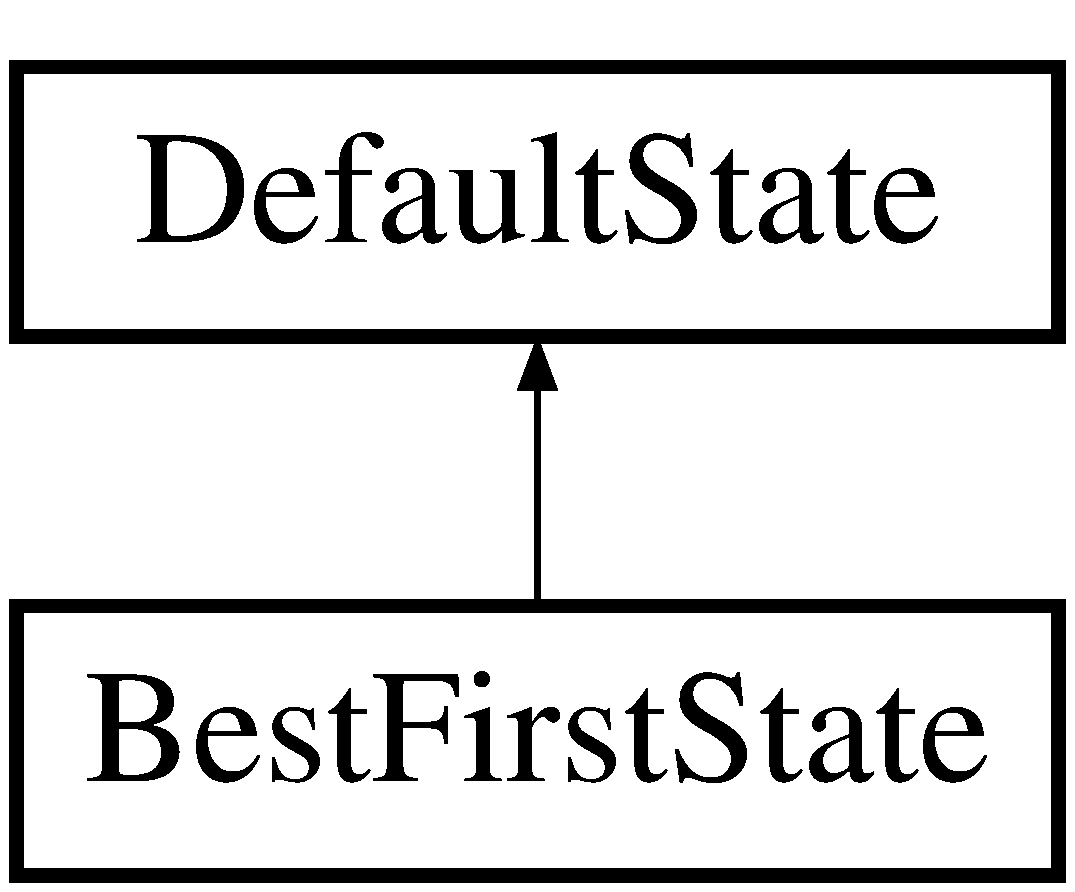
\includegraphics[height=2.000000cm]{class_best_first_state}
\end{center}
\end{figure}
\subsection*{Public Member Functions}
\begin{DoxyCompactItemize}
\item 
\hypertarget{class_best_first_state_a0704eec1c8b220625518dd2089247608}{{\bfseries Best\-First\-State} (Vector3 st)}\label{class_best_first_state_a0704eec1c8b220625518dd2089247608}

\item 
\hypertarget{class_best_first_state_a3353f52b010a1c812b28f58134a3c7bb}{override int {\bfseries Get\-Hash\-Code} ()}\label{class_best_first_state_a3353f52b010a1c812b28f58134a3c7bb}

\item 
\hypertarget{class_best_first_state_a286520962ee94165281a2a8f348761ce}{override bool {\bfseries Equals} (object obj)}\label{class_best_first_state_a286520962ee94165281a2a8f348761ce}

\item 
\hypertarget{class_best_first_state_aeecb81a2451e5b056a7a4b1cf4c2bbee}{bool {\bfseries Equals} (\hyperlink{class_best_first_state}{Best\-First\-State} obj)}\label{class_best_first_state_aeecb81a2451e5b056a7a4b1cf4c2bbee}

\item 
\hypertarget{class_best_first_state_a3d992e4922c88ef7d34b41598ac888a8}{override Vector3 {\bfseries state\-Position} ()}\label{class_best_first_state_a3d992e4922c88ef7d34b41598ac888a8}

\end{DoxyCompactItemize}
\subsection*{Public Attributes}
\begin{DoxyCompactItemize}
\item 
\hypertarget{class_best_first_state_af66fca05a46c3dfc43168d25eb609abb}{Vector3 {\bfseries state}}\label{class_best_first_state_af66fca05a46c3dfc43168d25eb609abb}

\end{DoxyCompactItemize}


The documentation for this class was generated from the following file\-:\begin{DoxyCompactItemize}
\item 
V\-A\-S\-T/vast/\-Assets/\-Plannar Scripts/\-Planners In Use/Best\-First\-Search\-Test.\-cs\end{DoxyCompactItemize}

\hypertarget{class_close_container}{\section{Close\-Container Class Reference}
\label{class_close_container}\index{Close\-Container@{Close\-Container}}
}
\subsection*{Public Member Functions}
\begin{DoxyCompactItemize}
\item 
\hyperlink{class_close_container_ac5d33c2ef7405e4dec717eb9cc5f049d}{Close\-Container} ()
\begin{DoxyCompactList}\small\item\em Initializes a new instance of the \hyperlink{class_close_container}{Close\-Container} class. \end{DoxyCompactList}\item 
void \hyperlink{class_close_container_a52aad3abda6bedf9ce5046cff5268c4b}{Insert} (\hyperlink{class_a_r_astar_node}{A\-R\-Astar\-Node} node)
\begin{DoxyCompactList}\small\item\em Inserts the specified node. \end{DoxyCompactList}\item 
List$<$ \hyperlink{class_default_state}{Default\-State} $>$ \hyperlink{class_close_container_a70df1c9c44b48239dec94bf34e3ddfcc}{keys} ()
\begin{DoxyCompactList}\small\item\em Returns a list with all keys in the dictionary. \end{DoxyCompactList}\item 
bool \hyperlink{class_close_container_af3fed08a9636b657f8f59512861aa095}{Contains} (\hyperlink{class_default_state}{Default\-State} state)
\begin{DoxyCompactList}\small\item\em Determines whether the container contains the specified state. \end{DoxyCompactList}\item 
Dictionary$<$ \hyperlink{class_default_state}{Default\-State}, \\*
\hyperlink{class_a_r_astar_node}{A\-R\-Astar\-Node} $>$ \hyperlink{class_close_container_ac18391d6d973ff76bc10346a7b469257}{Elements} ()
\begin{DoxyCompactList}\small\item\em Returns all elements in the container. \end{DoxyCompactList}\item 
void \hyperlink{class_close_container_accb0cc8ad39d76277547978e7bbd5ffb}{Clear} ()
\begin{DoxyCompactList}\small\item\em Clear all elements. \end{DoxyCompactList}\item 
void \hyperlink{class_close_container_ac058e024cd9b0a16d62ea660b6991bcb}{Update\-References} (float inflation\-Factor, \hyperlink{class_planning_domain_base}{Planning\-Domain\-Base} domain)
\begin{DoxyCompactList}\small\item\em Updates the references. \end{DoxyCompactList}\end{DoxyCompactItemize}


\subsection{Detailed Description}
This class represents the close list and provides abstraction for all the necesary functionality 

\subsection{Constructor \& Destructor Documentation}
\hypertarget{class_close_container_ac5d33c2ef7405e4dec717eb9cc5f049d}{\index{Close\-Container@{Close\-Container}!Close\-Container@{Close\-Container}}
\index{Close\-Container@{Close\-Container}!CloseContainer@{Close\-Container}}
\subsubsection[{Close\-Container}]{\setlength{\rightskip}{0pt plus 5cm}Close\-Container.\-Close\-Container (
\begin{DoxyParamCaption}
{}
\end{DoxyParamCaption}
)}}\label{class_close_container_ac5d33c2ef7405e4dec717eb9cc5f049d}


Initializes a new instance of the \hyperlink{class_close_container}{Close\-Container} class. 



\subsection{Member Function Documentation}
\hypertarget{class_close_container_accb0cc8ad39d76277547978e7bbd5ffb}{\index{Close\-Container@{Close\-Container}!Clear@{Clear}}
\index{Clear@{Clear}!CloseContainer@{Close\-Container}}
\subsubsection[{Clear}]{\setlength{\rightskip}{0pt plus 5cm}void Close\-Container.\-Clear (
\begin{DoxyParamCaption}
{}
\end{DoxyParamCaption}
)}}\label{class_close_container_accb0cc8ad39d76277547978e7bbd5ffb}


Clear all elements. 

\hypertarget{class_close_container_af3fed08a9636b657f8f59512861aa095}{\index{Close\-Container@{Close\-Container}!Contains@{Contains}}
\index{Contains@{Contains}!CloseContainer@{Close\-Container}}
\subsubsection[{Contains}]{\setlength{\rightskip}{0pt plus 5cm}bool Close\-Container.\-Contains (
\begin{DoxyParamCaption}
\item[{{\bf Default\-State}}]{state}
\end{DoxyParamCaption}
)}}\label{class_close_container_af3fed08a9636b657f8f59512861aa095}


Determines whether the container contains the specified state. 


\begin{DoxyParams}{Parameters}
{\em state} & The state we are checking for. \\
\hline
\end{DoxyParams}
\hypertarget{class_close_container_ac18391d6d973ff76bc10346a7b469257}{\index{Close\-Container@{Close\-Container}!Elements@{Elements}}
\index{Elements@{Elements}!CloseContainer@{Close\-Container}}
\subsubsection[{Elements}]{\setlength{\rightskip}{0pt plus 5cm}Dictionary$<${\bf Default\-State}, {\bf A\-R\-Astar\-Node}$>$ Close\-Container.\-Elements (
\begin{DoxyParamCaption}
{}
\end{DoxyParamCaption}
)}}\label{class_close_container_ac18391d6d973ff76bc10346a7b469257}


Returns all elements in the container. 

\hypertarget{class_close_container_a52aad3abda6bedf9ce5046cff5268c4b}{\index{Close\-Container@{Close\-Container}!Insert@{Insert}}
\index{Insert@{Insert}!CloseContainer@{Close\-Container}}
\subsubsection[{Insert}]{\setlength{\rightskip}{0pt plus 5cm}void Close\-Container.\-Insert (
\begin{DoxyParamCaption}
\item[{{\bf A\-R\-Astar\-Node}}]{node}
\end{DoxyParamCaption}
)}}\label{class_close_container_a52aad3abda6bedf9ce5046cff5268c4b}


Inserts the specified node. 


\begin{DoxyParams}{Parameters}
{\em node} & The node to be inserted \\
\hline
\end{DoxyParams}
\hypertarget{class_close_container_a70df1c9c44b48239dec94bf34e3ddfcc}{\index{Close\-Container@{Close\-Container}!keys@{keys}}
\index{keys@{keys}!CloseContainer@{Close\-Container}}
\subsubsection[{keys}]{\setlength{\rightskip}{0pt plus 5cm}List$<${\bf Default\-State}$>$ Close\-Container.\-keys (
\begin{DoxyParamCaption}
{}
\end{DoxyParamCaption}
)}}\label{class_close_container_a70df1c9c44b48239dec94bf34e3ddfcc}


Returns a list with all keys in the dictionary. 

\hypertarget{class_close_container_ac058e024cd9b0a16d62ea660b6991bcb}{\index{Close\-Container@{Close\-Container}!Update\-References@{Update\-References}}
\index{Update\-References@{Update\-References}!CloseContainer@{Close\-Container}}
\subsubsection[{Update\-References}]{\setlength{\rightskip}{0pt plus 5cm}void Close\-Container.\-Update\-References (
\begin{DoxyParamCaption}
\item[{float}]{inflation\-Factor, }
\item[{{\bf Planning\-Domain\-Base}}]{domain}
\end{DoxyParamCaption}
)}}\label{class_close_container_ac058e024cd9b0a16d62ea660b6991bcb}


Updates the references. 


\begin{DoxyParams}{Parameters}
{\em inflation\-Factor} & \hyperlink{class_planner}{Planner}'s current inflation factor. \\
\hline
{\em domain} & Current domain. \\
\hline
\end{DoxyParams}


The documentation for this class was generated from the following file\-:\begin{DoxyCompactItemize}
\item 
V\-A\-S\-T/vast/\-Assets/\-Plannar Scripts/\-Planners In Use/Containers.\-cs\end{DoxyCompactItemize}

\hypertarget{class_compare_costs}{\section{Compare\-Costs Class Reference}
\label{class_compare_costs}\index{Compare\-Costs@{Compare\-Costs}}
}


A functor class used to compare the costs of two Best\-First\-Search\-Nodes.  


\subsection*{Static Public Member Functions}
\begin{DoxyCompactItemize}
\item 
\hypertarget{class_compare_costs_af4215b898ea435febd8e80eb2bac6c7e}{static int {\bfseries Compare\-Cost} (\hyperlink{class_best_first_search_node}{Best\-First\-Search\-Node} n1, \hyperlink{class_best_first_search_node}{Best\-First\-Search\-Node} n2)}\label{class_compare_costs_af4215b898ea435febd8e80eb2bac6c7e}

\end{DoxyCompactItemize}


\subsection{Detailed Description}
A functor class used to compare the costs of two Best\-First\-Search\-Nodes. 

\begin{DoxySeeAlso}{See also}

\begin{DoxyItemize}
\item Documentation of the \hyperlink{class_best_first_search_planner}{Best\-First\-Search\-Planner} class, which describes how states and actions are used. 
\end{DoxyItemize}
\end{DoxySeeAlso}


The documentation for this class was generated from the following file\-:\begin{DoxyCompactItemize}
\item 
V\-A\-S\-T/vast/\-Assets/\-Plannar Scripts/\-Planners In Use/Best\-First\-Search\-Planner.\-cs\end{DoxyCompactItemize}

\hypertarget{class_default_action}{\section{Default\-Action Class Reference}
\label{class_default_action}\index{Default\-Action@{Default\-Action}}
}


The default class used to describe a transition between states, if it was not specified by the user.  


Inheritance diagram for Default\-Action\-:\begin{figure}[H]
\begin{center}
\leavevmode
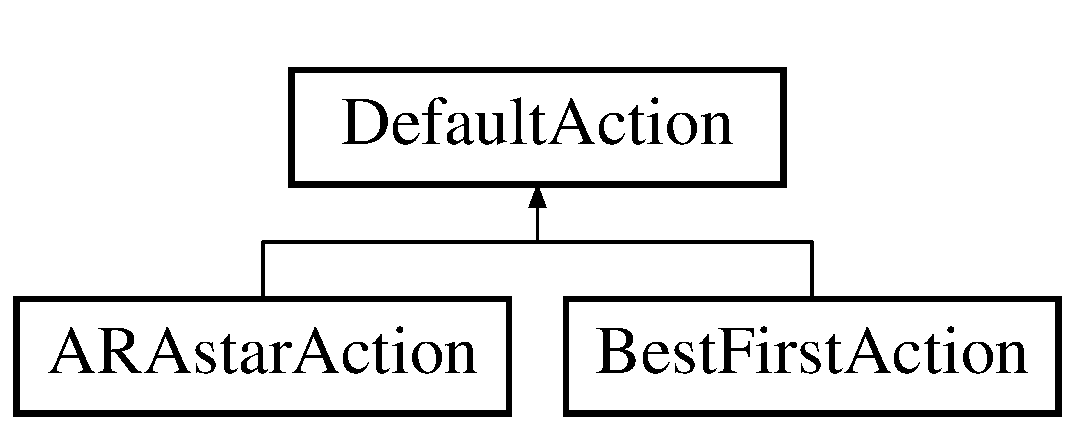
\includegraphics[height=2.000000cm]{class_default_action}
\end{center}
\end{figure}
\subsection*{Public Attributes}
\begin{DoxyCompactItemize}
\item 
\hypertarget{class_default_action_a1ccad71698500fe44418f8242854e4dc}{float {\bfseries cost}}\label{class_default_action_a1ccad71698500fe44418f8242854e4dc}

\item 
\hypertarget{class_default_action_ac8d9ed08df293eb8657051e181a68782}{\hyperlink{class_default_state}{Default\-State} {\bfseries state}}\label{class_default_action_ac8d9ed08df293eb8657051e181a68782}

\end{DoxyCompactItemize}


\subsection{Detailed Description}
The default class used to describe a transition between states, if it was not specified by the user. 

\begin{DoxySeeAlso}{See also}

\begin{DoxyItemize}
\item Documentation of the \hyperlink{class_best_first_search_planner}{Best\-First\-Search\-Planner} class, which describes how states and actions are used. 
\end{DoxyItemize}
\end{DoxySeeAlso}


The documentation for this class was generated from the following file\-:\begin{DoxyCompactItemize}
\item 
V\-A\-S\-T/vast/\-Assets/\-Plannar Scripts/\-Planners In Use/Best\-First\-Search\-Planner.\-cs\end{DoxyCompactItemize}

\hypertarget{class_default_state}{\section{Default\-State Class Reference}
\label{class_default_state}\index{Default\-State@{Default\-State}}
}
Inheritance diagram for Default\-State\-:\begin{figure}[H]
\begin{center}
\leavevmode
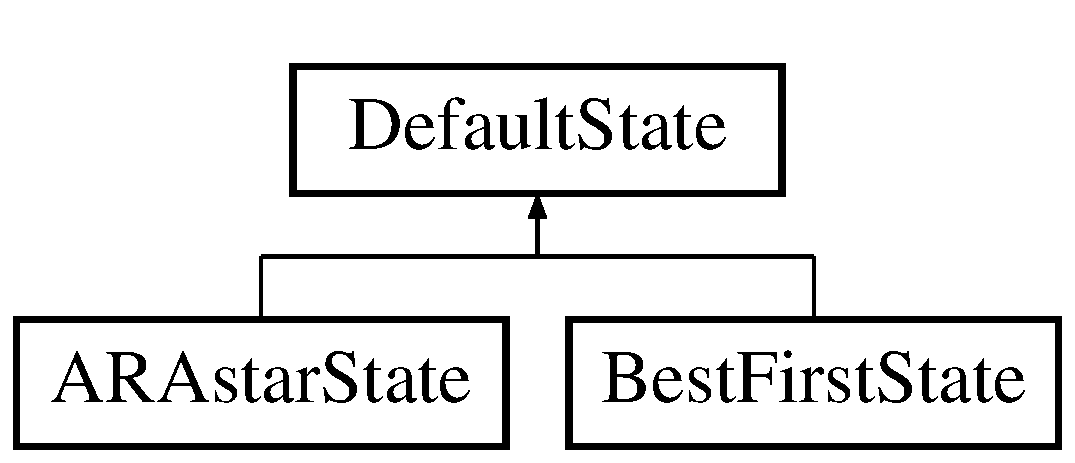
\includegraphics[height=2.000000cm]{class_default_state}
\end{center}
\end{figure}
\subsection*{Public Member Functions}
\begin{DoxyCompactItemize}
\item 
\hypertarget{class_default_state_a3091716e0c5026f23b55f1b377f27b6a}{virtual Vector3 {\bfseries state\-Position} ()}\label{class_default_state_a3091716e0c5026f23b55f1b377f27b6a}

\end{DoxyCompactItemize}


\subsection{Detailed Description}
Base class for deriving states 

The documentation for this class was generated from the following file\-:\begin{DoxyCompactItemize}
\item 
V\-A\-S\-T/vast/\-Assets/\-Plannar Scripts/\-Planners In Use/Best\-First\-Search\-Planner.\-cs\end{DoxyCompactItemize}

\hypertarget{class_grid_neighbors}{\section{Grid\-Neighbors Class Reference}
\label{class_grid_neighbors}\index{Grid\-Neighbors@{Grid\-Neighbors}}
}
Inheritance diagram for Grid\-Neighbors\-:\begin{figure}[H]
\begin{center}
\leavevmode
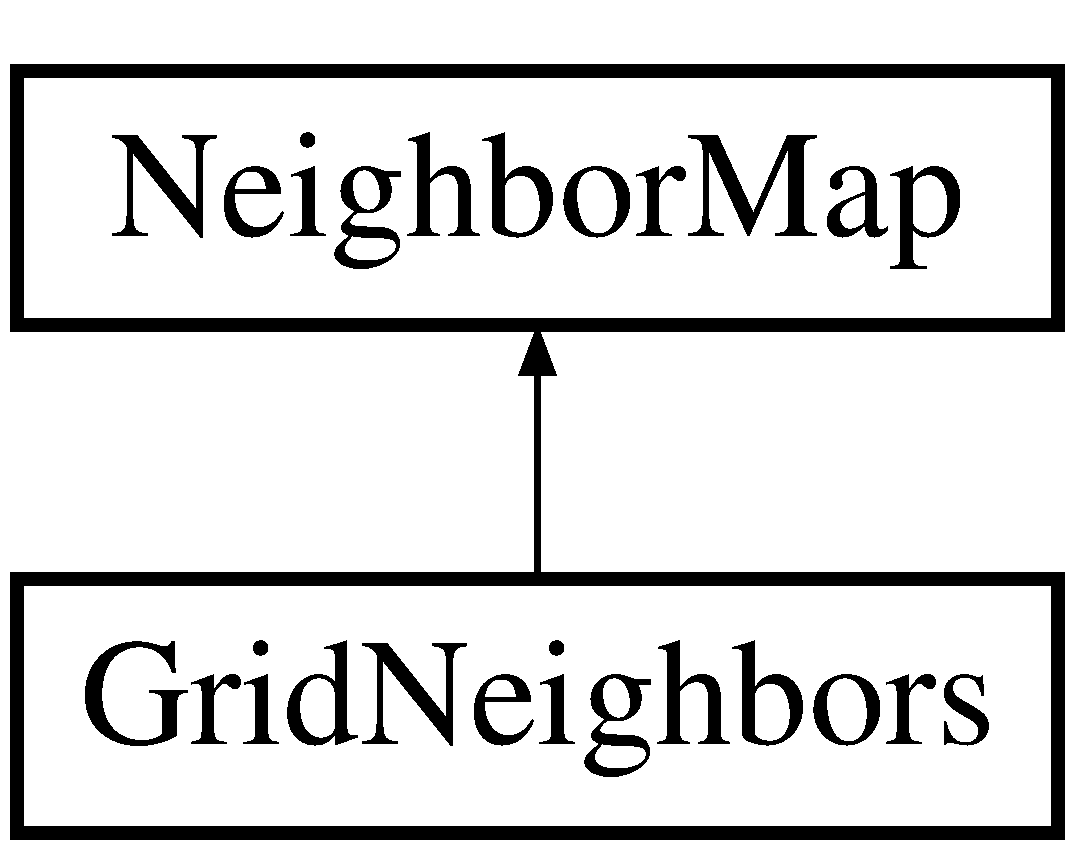
\includegraphics[height=2.000000cm]{class_grid_neighbors}
\end{center}
\end{figure}
\subsection*{Additional Inherited Members}


The documentation for this class was generated from the following file\-:\begin{DoxyCompactItemize}
\item 
V\-A\-S\-T/vast/\-Assets/\-Plannar Scripts/\-Planners In Use/A\-R\-Astar\-Test.\-cs\end{DoxyCompactItemize}

\hypertarget{class_incons}{\section{Incons Class Reference}
\label{class_incons}\index{Incons@{Incons}}
}
\subsection*{Public Member Functions}
\begin{DoxyCompactItemize}
\item 
\hyperlink{class_incons_a30350207d1df50ea95ea1a06f571a5fe}{Incons} ()
\begin{DoxyCompactList}\small\item\em Initializes a new instance of the \hyperlink{class_incons}{Incons} class. \end{DoxyCompactList}\item 
void \hyperlink{class_incons_a599de106ff55f34789e0d5140eabfe48}{Insert} (\hyperlink{class_a_r_astar_node}{A\-R\-Astar\-Node} node)
\begin{DoxyCompactList}\small\item\em Insert the specified node. \end{DoxyCompactList}\item 
Dictionary$<$ \hyperlink{class_default_state}{Default\-State}, \\*
\hyperlink{class_a_r_astar_node}{A\-R\-Astar\-Node} $>$ \hyperlink{class_incons_a728bdf34ed93795bcf20e77ff01ef23d}{Elements} ()
\begin{DoxyCompactList}\small\item\em Returns all de elements in the container. \end{DoxyCompactList}\item 
List$<$ \hyperlink{class_default_state}{Default\-State} $>$ \hyperlink{class_incons_af233952cd9fa9a2c7478bc02c29e3aad}{keys} ()
\begin{DoxyCompactList}\small\item\em Returns a list with all statttes in the container. \end{DoxyCompactList}\item 
void \hyperlink{class_incons_aa9e20464feb57c967621d58319d88f5e}{Move\-To\-Open} (ref \hyperlink{class_open_container}{Open\-Container} open)
\begin{DoxyCompactList}\small\item\em Moves nodes to open. \end{DoxyCompactList}\item 
void \hyperlink{class_incons_a50eda8dae76cbdc9d30e4ecef8645a8b}{Clear} ()
\begin{DoxyCompactList}\small\item\em Clear all nodes in the container. \end{DoxyCompactList}\end{DoxyCompactItemize}


\subsection{Detailed Description}
This class represents the inconsistent list. It provides abstraction for all the necessary functionality 

\subsection{Constructor \& Destructor Documentation}
\hypertarget{class_incons_a30350207d1df50ea95ea1a06f571a5fe}{\index{Incons@{Incons}!Incons@{Incons}}
\index{Incons@{Incons}!Incons@{Incons}}
\subsubsection[{Incons}]{\setlength{\rightskip}{0pt plus 5cm}Incons.\-Incons (
\begin{DoxyParamCaption}
{}
\end{DoxyParamCaption}
)}}\label{class_incons_a30350207d1df50ea95ea1a06f571a5fe}


Initializes a new instance of the \hyperlink{class_incons}{Incons} class. 



\subsection{Member Function Documentation}
\hypertarget{class_incons_a50eda8dae76cbdc9d30e4ecef8645a8b}{\index{Incons@{Incons}!Clear@{Clear}}
\index{Clear@{Clear}!Incons@{Incons}}
\subsubsection[{Clear}]{\setlength{\rightskip}{0pt plus 5cm}void Incons.\-Clear (
\begin{DoxyParamCaption}
{}
\end{DoxyParamCaption}
)}}\label{class_incons_a50eda8dae76cbdc9d30e4ecef8645a8b}


Clear all nodes in the container. 

\hypertarget{class_incons_a728bdf34ed93795bcf20e77ff01ef23d}{\index{Incons@{Incons}!Elements@{Elements}}
\index{Elements@{Elements}!Incons@{Incons}}
\subsubsection[{Elements}]{\setlength{\rightskip}{0pt plus 5cm}Dictionary$<${\bf Default\-State}, {\bf A\-R\-Astar\-Node}$>$ Incons.\-Elements (
\begin{DoxyParamCaption}
{}
\end{DoxyParamCaption}
)}}\label{class_incons_a728bdf34ed93795bcf20e77ff01ef23d}


Returns all de elements in the container. 

\hypertarget{class_incons_a599de106ff55f34789e0d5140eabfe48}{\index{Incons@{Incons}!Insert@{Insert}}
\index{Insert@{Insert}!Incons@{Incons}}
\subsubsection[{Insert}]{\setlength{\rightskip}{0pt plus 5cm}void Incons.\-Insert (
\begin{DoxyParamCaption}
\item[{{\bf A\-R\-Astar\-Node}}]{node}
\end{DoxyParamCaption}
)}}\label{class_incons_a599de106ff55f34789e0d5140eabfe48}


Insert the specified node. 


\begin{DoxyParams}{Parameters}
{\em node} & Node to be inserted. \\
\hline
\end{DoxyParams}
\hypertarget{class_incons_af233952cd9fa9a2c7478bc02c29e3aad}{\index{Incons@{Incons}!keys@{keys}}
\index{keys@{keys}!Incons@{Incons}}
\subsubsection[{keys}]{\setlength{\rightskip}{0pt plus 5cm}List$<${\bf Default\-State}$>$ Incons.\-keys (
\begin{DoxyParamCaption}
{}
\end{DoxyParamCaption}
)}}\label{class_incons_af233952cd9fa9a2c7478bc02c29e3aad}


Returns a list with all statttes in the container. 

\hypertarget{class_incons_aa9e20464feb57c967621d58319d88f5e}{\index{Incons@{Incons}!Move\-To\-Open@{Move\-To\-Open}}
\index{Move\-To\-Open@{Move\-To\-Open}!Incons@{Incons}}
\subsubsection[{Move\-To\-Open}]{\setlength{\rightskip}{0pt plus 5cm}void Incons.\-Move\-To\-Open (
\begin{DoxyParamCaption}
\item[{ref {\bf Open\-Container}}]{open}
\end{DoxyParamCaption}
)}}\label{class_incons_aa9e20464feb57c967621d58319d88f5e}


Moves nodes to open. 


\begin{DoxyParams}{Parameters}
{\em open} & A reference to the open container. \\
\hline
\end{DoxyParams}


The documentation for this class was generated from the following file\-:\begin{DoxyCompactItemize}
\item 
V\-A\-S\-T/vast/\-Assets/\-Plannar Scripts/\-Planners In Use/Containers.\-cs\end{DoxyCompactItemize}

\hypertarget{interface_i_planner_interface-g}{\section{I\-Planner\-Interface$<$ State\-Map $>$ Interface Template Reference}
\label{interface_i_planner_interface-g}\index{I\-Planner\-Interface$<$ State\-Map $>$@{I\-Planner\-Interface$<$ State\-Map $>$}}
}
\subsection*{Public Member Functions}
\begin{DoxyCompactItemize}
\item 
\hypertarget{interface_i_planner_interface-g_af03854cd5c2754a5786f756047e70ef4}{void {\bfseries init} (ref List$<$ \hyperlink{class_planning_domain_base}{Planning\-Domain\-Base} $>$ new\-Planning\-Domain, int max\-Num\-Nodes\-To\-Expand)}\label{interface_i_planner_interface-g_af03854cd5c2754a5786f756047e70ef4}

\item 
\hypertarget{interface_i_planner_interface-g_a0e234718e6fe3da7addf43003d40693f}{bool {\bfseries \-\_\-compute\-Plan} (ref \hyperlink{class_default_state}{Default\-State} start\-State, ref \hyperlink{class_default_state}{Default\-State} ideal\-Goal\-State, State\-Map map, ref \hyperlink{class_default_state}{Default\-State} actual\-State\-Reached, float max\-Time)}\label{interface_i_planner_interface-g_a0e234718e6fe3da7addf43003d40693f}

\end{DoxyCompactItemize}


The documentation for this interface was generated from the following file\-:\begin{DoxyCompactItemize}
\item 
V\-A\-S\-T/vast/\-Assets/\-Plannar Scripts/\-Planners In Use/Best\-First\-Search\-Planner.\-cs\end{DoxyCompactItemize}

\hypertarget{class_neighbor_map}{\section{Neighbor\-Map Class Reference}
\label{class_neighbor_map}\index{Neighbor\-Map@{Neighbor\-Map}}
}
Inheritance diagram for Neighbor\-Map\-:\begin{figure}[H]
\begin{center}
\leavevmode
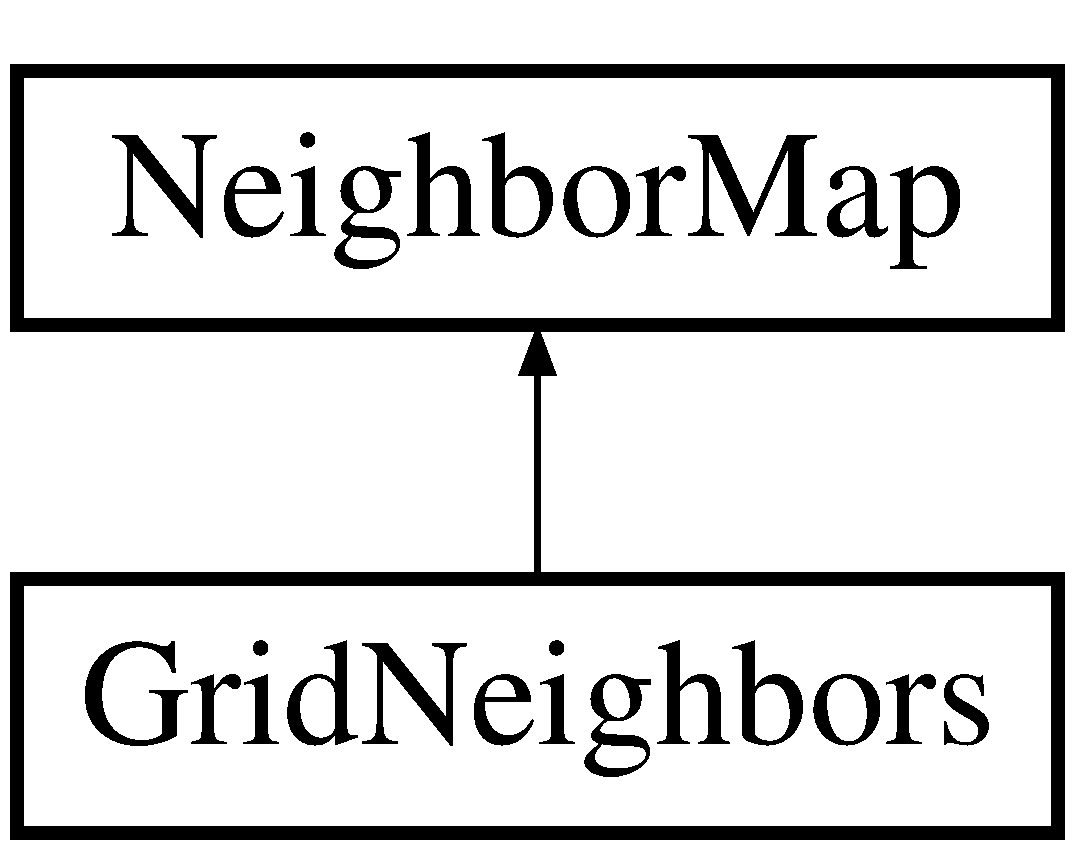
\includegraphics[height=2.000000cm]{class_neighbor_map}
\end{center}
\end{figure}
\subsection*{Public Attributes}
\begin{DoxyCompactItemize}
\item 
\hypertarget{class_neighbor_map_a420488d93080691ce0dd6791a48d817c}{Dictionary$<$ \hyperlink{class_default_state}{Default\-State}, List\\*
$<$ \hyperlink{class_default_state}{Default\-State} $>$ $>$ {\bfseries neighbor\-Map}}\label{class_neighbor_map_a420488d93080691ce0dd6791a48d817c}

\end{DoxyCompactItemize}


The documentation for this class was generated from the following file\-:\begin{DoxyCompactItemize}
\item 
V\-A\-S\-T/vast/\-Assets/\-Plannar Scripts/\-Planners In Use/A\-R\-Astar\-Test.\-cs\end{DoxyCompactItemize}

\hypertarget{class_node_comparer}{\section{Node\-Comparer Class Reference}
\label{class_node_comparer}\index{Node\-Comparer@{Node\-Comparer}}
}
\subsection*{Public Member Functions}
\begin{DoxyCompactItemize}
\item 
\hypertarget{class_node_comparer_ae9d57c1351837629d2227a952a580326}{{\bfseries Node\-Comparer} (\hyperlink{class_a_r_astar_planner}{A\-R\-Astar\-Planner} planner)}\label{class_node_comparer_ae9d57c1351837629d2227a952a580326}

\item 
\hypertarget{class_node_comparer_a1d1cc1dcf638d05f91398876ab8ba4b2}{int {\bfseries Compare} (\hyperlink{class_a_r_astar_node}{A\-R\-Astar\-Node} n1, \hyperlink{class_a_r_astar_node}{A\-R\-Astar\-Node} n2)}\label{class_node_comparer_a1d1cc1dcf638d05f91398876ab8ba4b2}

\end{DoxyCompactItemize}


The documentation for this class was generated from the following file\-:\begin{DoxyCompactItemize}
\item 
V\-A\-S\-T/vast/\-Assets/\-Plannar Scripts/\-Planners In Use/A\-R\-Astar\-Node.\-cs\end{DoxyCompactItemize}

\hypertarget{class_open_container}{\section{Open\-Container Class Reference}
\label{class_open_container}\index{Open\-Container@{Open\-Container}}
}
\subsection*{Public Member Functions}
\begin{DoxyCompactItemize}
\item 
\hypertarget{class_open_container_a8fe6042f8f2b6e023c0ccbeb302c3145}{{\bfseries Open\-Container} (\hyperlink{class_a_r_astar_planner}{A\-R\-Astar\-Planner} planner, \hyperlink{class_planning_domain_base}{Planning\-Domain\-Base} \-\_\-domain, bool \-\_\-use\-Heap=true)}\label{class_open_container_a8fe6042f8f2b6e023c0ccbeb302c3145}

\item 
\hypertarget{class_open_container_a9c2ac72d426256bd0f038b7375fb184e}{List$<$ \hyperlink{class_default_state}{Default\-State} $>$ {\bfseries keys} ()}\label{class_open_container_a9c2ac72d426256bd0f038b7375fb184e}

\item 
\hypertarget{class_open_container_ab7eb3e91880b999b099b54c4325dcec9}{Dictionary$<$ \hyperlink{class_default_state}{Default\-State}, \\*
\hyperlink{class_a_r_astar_node}{A\-R\-Astar\-Node} $>$ {\bfseries Elements} ()}\label{class_open_container_ab7eb3e91880b999b099b54c4325dcec9}

\item 
\hypertarget{class_open_container_a9f4b0b441dba986b7bf15d9359eb6900}{void {\bfseries clear\-High\-Priority} ()}\label{class_open_container_a9f4b0b441dba986b7bf15d9359eb6900}

\item 
\hypertarget{class_open_container_ad8c27e3618b6988966c38fe76cc87e65}{\hyperlink{class_a_r_astar_node}{A\-R\-Astar\-Node} {\bfseries Node} (\hyperlink{class_default_state}{Default\-State} state)}\label{class_open_container_ad8c27e3618b6988966c38fe76cc87e65}

\item 
\hypertarget{class_open_container_a19e53059762a7f0aa5bb5a96fe31506d}{\hyperlink{class_a_r_astar_node}{A\-R\-Astar\-Node} {\bfseries First} ()}\label{class_open_container_a19e53059762a7f0aa5bb5a96fe31506d}

\item 
\hypertarget{class_open_container_abd9ac817ab140603feee84f8995a27a0}{int {\bfseries List\-Count} ()}\label{class_open_container_abd9ac817ab140603feee84f8995a27a0}

\item 
\hypertarget{class_open_container_a5f585b8681b2e0425119f7a59caf362e}{void {\bfseries Remove} (\hyperlink{class_default_state}{Default\-State} state)}\label{class_open_container_a5f585b8681b2e0425119f7a59caf362e}

\item 
\hypertarget{class_open_container_a3cd8532faf8cf40de6b89fb57c685df8}{void {\bfseries Insert} (\hyperlink{class_a_r_astar_node}{A\-R\-Astar\-Node} node)}\label{class_open_container_a3cd8532faf8cf40de6b89fb57c685df8}

\item 
\hypertarget{class_open_container_a09946014eab624c239cce93a85988071}{void {\bfseries Sort} ()}\label{class_open_container_a09946014eab624c239cce93a85988071}

\item 
\hypertarget{class_open_container_ac3edc61c5f1a9b66c3f7c7acd0640e0d}{void {\bfseries Update\-List} (\hyperlink{class_a_r_astar_node}{A\-R\-Astar\-Node} current\-State)}\label{class_open_container_ac3edc61c5f1a9b66c3f7c7acd0640e0d}

\item 
\hypertarget{class_open_container_a12984d3becd0ff24eca4c4371881a71b}{void {\bfseries Update\-Heuristic} (\hyperlink{class_default_state}{Default\-State} goal)}\label{class_open_container_a12984d3becd0ff24eca4c4371881a71b}

\item 
\hypertarget{class_open_container_ae5ef558400b142f682464bdab1174e43}{bool {\bfseries Contains\-State} (\hyperlink{class_default_state}{Default\-State} state)}\label{class_open_container_ae5ef558400b142f682464bdab1174e43}

\end{DoxyCompactItemize}
\subsection*{Public Attributes}
\begin{DoxyCompactItemize}
\item 
\hypertarget{class_open_container_a656a492f930544d2691fa1780cc14e26}{\hyperlink{class_default_state}{Default\-State} {\bfseries start\-State}}\label{class_open_container_a656a492f930544d2691fa1780cc14e26}

\end{DoxyCompactItemize}


The documentation for this class was generated from the following file\-:\begin{DoxyCompactItemize}
\item 
V\-A\-S\-T/vast/\-Assets/\-Plannar Scripts/\-Planners In Use/Containers.\-cs\end{DoxyCompactItemize}

\hypertarget{class_plan_container}{\section{Plan\-Container Class Reference}
\label{class_plan_container}\index{Plan\-Container@{Plan\-Container}}
}
\subsection*{Public Member Functions}
\begin{DoxyCompactItemize}
\item 
\hypertarget{class_plan_container_af4eac8ba49af8845098657fbce70bd5c}{{\bfseries Plan\-Container} (Dictionary$<$ \hyperlink{class_default_state}{Default\-State}, \hyperlink{class_a_r_astar_node}{A\-R\-Astar\-Node} $>$ \-\_\-plan)}\label{class_plan_container_af4eac8ba49af8845098657fbce70bd5c}

\item 
\hypertarget{class_plan_container_a1c5b054eddfff18de7d02631a4babdfd}{\hyperlink{class_a_r_astar_node}{A\-R\-Astar\-Node} {\bfseries Node} (\hyperlink{class_default_state}{Default\-State} st)}\label{class_plan_container_a1c5b054eddfff18de7d02631a4babdfd}

\item 
\hypertarget{class_plan_container_a7fd7f8b92671e2a0f64d2bde1b508809}{void {\bfseries Remove} (\hyperlink{class_default_state}{Default\-State} state)}\label{class_plan_container_a7fd7f8b92671e2a0f64d2bde1b508809}

\item 
\hypertarget{class_plan_container_a055275bf8a2330996670c669ec23f89f}{void {\bfseries Insert\-Node} (ref \hyperlink{class_default_state}{Default\-State} st, ref \hyperlink{class_a_r_astar_node}{A\-R\-Astar\-Node} node)}\label{class_plan_container_a055275bf8a2330996670c669ec23f89f}

\item 
\hypertarget{class_plan_container_a91e41d4fd5a34c3cf958f0940dfb8d10}{void {\bfseries Update\-Costs} (float cost)}\label{class_plan_container_a91e41d4fd5a34c3cf958f0940dfb8d10}

\item 
\hypertarget{class_plan_container_a16e1e615e844f1164867046b526b3ef1}{void {\bfseries Update\-Heuristic} (\hyperlink{class_default_state}{Default\-State} goal)}\label{class_plan_container_a16e1e615e844f1164867046b526b3ef1}

\item 
\hypertarget{class_plan_container_a317026e533d9ccc429cc7552cbaf0a86}{Dictionary$<$ \hyperlink{class_default_state}{Default\-State}, \\*
\hyperlink{class_a_r_astar_node}{A\-R\-Astar\-Node} $>$ {\bfseries Elements} ()}\label{class_plan_container_a317026e533d9ccc429cc7552cbaf0a86}

\item 
\hypertarget{class_plan_container_aaae2bc99a50902c06aeb128b9152b4f0}{void {\bfseries Fill} (ref \hyperlink{class_close_container}{Close\-Container} Close, Dictionary$<$ \hyperlink{class_default_state}{Default\-State}, \hyperlink{class_a_r_astar_node}{A\-R\-Astar\-Node} $>$ Visited, ref \hyperlink{class_default_state}{Default\-State} state\-Reached, \hyperlink{class_planning_domain_base}{Planning\-Domain\-Base} domain, ref \hyperlink{class_default_state}{Default\-State} current, ref Key\-Value\-Pair$<$ \hyperlink{class_default_state}{Default\-State}, \hyperlink{class_a_r_astar_node}{A\-R\-Astar\-Node} $>$ goal\-Pair, float inflation\-Factor)}\label{class_plan_container_aaae2bc99a50902c06aeb128b9152b4f0}

\item 
\hypertarget{class_plan_container_a49a5878c3e1d12926d9bac5b93ab8fbc}{bool {\bfseries Contains\-State} (\hyperlink{class_default_state}{Default\-State} state)}\label{class_plan_container_a49a5878c3e1d12926d9bac5b93ab8fbc}

\item 
\hypertarget{class_plan_container_a16479b9695345f4ca9385f85f4632716}{void {\bfseries Clear} ()}\label{class_plan_container_a16479b9695345f4ca9385f85f4632716}

\end{DoxyCompactItemize}


The documentation for this class was generated from the following file\-:\begin{DoxyCompactItemize}
\item 
V\-A\-S\-T/vast/\-Assets/\-Plannar Scripts/\-Planners In Use/Containers.\-cs\end{DoxyCompactItemize}

\hypertarget{class_planner}{\section{Planner Class Reference}
\label{class_planner}\index{Planner@{Planner}}
}
\subsection*{Public Member Functions}
\begin{DoxyCompactItemize}
\item 
\hypertarget{class_planner_a547ab7ac5131f9a7b1c21a2c0315a9a5}{virtual Footstep\-Planning\-Action\mbox{[}$\,$\mbox{]} {\bfseries Get\-Output\-Plan} ()}\label{class_planner_a547ab7ac5131f9a7b1c21a2c0315a9a5}

\item 
\hypertarget{class_planner_a524224551fd946ebbdd3ed63fe3a6403}{virtual bool {\bfseries Is\-Empty} ()}\label{class_planner_a524224551fd946ebbdd3ed63fe3a6403}

\item 
\hypertarget{class_planner_a45faf2988ce1bb00355579b2d1db6545}{virtual bool {\bfseries Has\-Expired} ()}\label{class_planner_a45faf2988ce1bb00355579b2d1db6545}

\item 
\hypertarget{class_planner_ad0954ae572578966463be213f396ed78}{virtual bool {\bfseries There\-Still\-Time} ()}\label{class_planner_ad0954ae572578966463be213f396ed78}

\item 
\hypertarget{class_planner_ae9528547234832c67b351e6800b94ff5}{virtual void {\bfseries Recompute\-Plan} ()}\label{class_planner_ae9528547234832c67b351e6800b94ff5}

\item 
\hypertarget{class_planner_a223b6149af3af1f6ba2e61e51e6dda87}{virtual void {\bfseries Init} (Animation\-Analyzer aa, Neighbour\-Agents na, Neighbour\-Obstacles no)}\label{class_planner_a223b6149af3af1f6ba2e61e51e6dda87}

\item 
\hypertarget{class_planner_acbe375938802581e5338e61145711ca0}{virtual int {\bfseries Get\-Number\-Of\-Domains} ()}\label{class_planner_acbe375938802581e5338e61145711ca0}

\item 
\hypertarget{class_planner_ab8dcacec087454aec674af4380286bba}{virtual bool {\bfseries Check\-Domain\-State\-Collisions} (int d, Footstep\-Planning\-State st)}\label{class_planner_ab8dcacec087454aec674af4380286bba}

\item 
\hypertarget{class_planner_a9d3ca9d667c8330d241fcc61d5b2e8f5}{virtual bool {\bfseries Compute\-Plan} ()}\label{class_planner_a9d3ca9d667c8330d241fcc61d5b2e8f5}

\item 
\hypertarget{class_planner_a599560668fe905b64d30794632169945}{virtual Footstep\-Planning\-Action {\bfseries get\-First\-Action} ()}\label{class_planner_a599560668fe905b64d30794632169945}

\end{DoxyCompactItemize}
\subsection*{Public Attributes}
\begin{DoxyCompactItemize}
\item 
\hypertarget{class_planner_a61bc5fb92926adb1d47117b3953dc838}{float {\bfseries goal\-Time}}\label{class_planner_a61bc5fb92926adb1d47117b3953dc838}

\item 
\hypertarget{class_planner_a11545a956f32850f9bee31866e6c1854}{int {\bfseries Max\-Number\-Of\-Nodes}}\label{class_planner_a11545a956f32850f9bee31866e6c1854}

\item 
\hypertarget{class_planner_a25d7f8ac309c61b0c1f161c36b771a6d}{float {\bfseries max\-Time}}\label{class_planner_a25d7f8ac309c61b0c1f161c36b771a6d}

\item 
\hypertarget{class_planner_a935d9d44e2bf7cfb086aef8a4a272893}{Transform {\bfseries root}}\label{class_planner_a935d9d44e2bf7cfb086aef8a4a272893}

\item 
\hypertarget{class_planner_a15508936d815ce9a6cd111428e6ed819}{Transform {\bfseries current\-State\-Transform}}\label{class_planner_a15508936d815ce9a6cd111428e6ed819}

\item 
\hypertarget{class_planner_a30a77ede048aecc823adc2775718df2a}{Transform {\bfseries goal\-State\-Transform}}\label{class_planner_a30a77ede048aecc823adc2775718df2a}

\item 
\hypertarget{class_planner_af95edfb9e8e93af5dccf7e6b18d7a9c6}{Vector3 {\bfseries current\-Goal}}\label{class_planner_af95edfb9e8e93af5dccf7e6b18d7a9c6}

\item 
\hypertarget{class_planner_a752390ecc83a78028b2ec28efe5b9d34}{Material {\bfseries goal\-Completed\-Material}}\label{class_planner_a752390ecc83a78028b2ec28efe5b9d34}

\item 
\hypertarget{class_planner_aead3ef24c43c10820e48e51ae21d3280}{Material {\bfseries goal\-Material}}\label{class_planner_aead3ef24c43c10820e48e51ae21d3280}

\item 
\hypertarget{class_planner_aee6e18d65f96ef4b7bfdc7fc035c5d43}{Footstep\-Planning\-State {\bfseries current\-State}}\label{class_planner_aee6e18d65f96ef4b7bfdc7fc035c5d43}

\item 
\hypertarget{class_planner_ab9722eb37c59037b8ee255d129714b62}{bool {\bfseries initialized}}\label{class_planner_ab9722eb37c59037b8ee255d129714b62}

\item 
\hypertarget{class_planner_a73e7ae359b3f55578281abd81efecae1}{bool {\bfseries is\-Plan\-Computed}}\label{class_planner_a73e7ae359b3f55578281abd81efecae1}

\item 
\hypertarget{class_planner_a665a17a87d386ae4b9caa47633e06a24}{bool {\bfseries plan\-Changed}}\label{class_planner_a665a17a87d386ae4b9caa47633e06a24}

\item 
\hypertarget{class_planner_a26d738b32b82068c03b47eba1f6d8c0d}{bool {\bfseries goal\-Reached}}\label{class_planner_a26d738b32b82068c03b47eba1f6d8c0d}

\end{DoxyCompactItemize}


The documentation for this class was generated from the following file\-:\begin{DoxyCompactItemize}
\item 
V\-A\-S\-T/vast/\-Assets/\-Plannar Scripts/\-Planners In Use/Best\-First\-Search\-Planner.\-cs\end{DoxyCompactItemize}

\hypertarget{class_planning_domain_base}{\section{Planning\-Domain\-Base Class Reference}
\label{class_planning_domain_base}\index{Planning\-Domain\-Base@{Planning\-Domain\-Base}}
}


A base class for implementing a planning domain used by the \hyperlink{class_best_first_search_planner}{Best\-First\-Search\-Planner}.  


Inheritance diagram for Planning\-Domain\-Base\-:\begin{figure}[H]
\begin{center}
\leavevmode
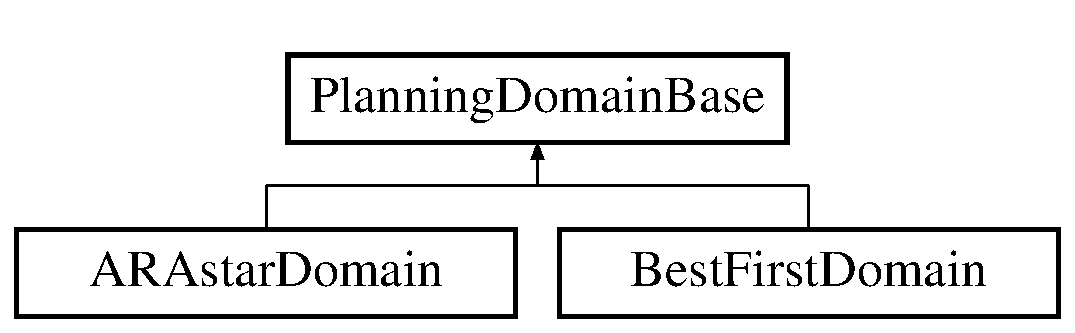
\includegraphics[height=2.000000cm]{class_planning_domain_base}
\end{center}
\end{figure}
\subsection*{Public Member Functions}
\begin{DoxyCompactItemize}
\item 
virtual bool \hyperlink{class_planning_domain_base_a56907006c1e4a4071f58da65705792d1}{is\-A\-Goal\-State} (ref \hyperlink{class_default_state}{Default\-State} state, ref \hyperlink{class_default_state}{Default\-State} ideal\-Goal\-State)
\begin{DoxyCompactList}\small\item\em Returns true if state is a valid goal state for the planning problem. \end{DoxyCompactList}\item 
virtual void \hyperlink{class_planning_domain_base_adbca97ccf882076eb737b8bebf1fb1ea}{generate\-Transitions} (ref \hyperlink{class_default_state}{Default\-State} current\-State, ref \hyperlink{class_default_state}{Default\-State} previous\-State, ref \hyperlink{class_default_state}{Default\-State} ideal\-Goal\-State, ref List$<$ \hyperlink{class_default_action}{Default\-Action} $>$ transitions)
\begin{DoxyCompactList}\small\item\em Populates the list of actions that can be taken from the current state. \end{DoxyCompactList}\item 
\hypertarget{class_planning_domain_base_ac045b562142c74659dd0624ae38f670e}{virtual void {\bfseries generate\-Neighbors} (\hyperlink{class_default_state}{Default\-State} current\-State, ref List$<$ \hyperlink{class_default_state}{Default\-State} $>$ neighbors)}\label{class_planning_domain_base_ac045b562142c74659dd0624ae38f670e}

\item 
\hypertarget{class_planning_domain_base_a94174e0d5948bd2b8f611a36050fcc95}{virtual void {\bfseries generate\-Predecessors} (\hyperlink{class_default_state}{Default\-State} current\-State, ref List$<$ \hyperlink{class_default_action}{Default\-Action} $>$ action\-List)}\label{class_planning_domain_base_a94174e0d5948bd2b8f611a36050fcc95}

\item 
virtual float \hyperlink{class_planning_domain_base_a4d0f803c0d3dfb3f59526078db674a4f}{estimate\-Total\-Cost} (ref \hyperlink{class_default_state}{Default\-State} current\-State, ref \hyperlink{class_default_state}{Default\-State} ideal\-Goal\-State, float currentg)
\begin{DoxyCompactList}\small\item\em Computes the heuristic function (often denoted as f) that estimates the \char`\"{}goodness\char`\"{} of a state towards the goal. \end{DoxyCompactList}\item 
\hypertarget{class_planning_domain_base_a123435365f69b0c6969b3c69f05fb007}{virtual float {\bfseries evaluate\-Domain} (ref \hyperlink{class_default_state}{Default\-State} state)}\label{class_planning_domain_base_a123435365f69b0c6969b3c69f05fb007}

\item 
\hypertarget{class_planning_domain_base_a07faaa66f466a9d7ce3c4ffe37e62984}{virtual bool {\bfseries Check\-State\-Collisions} (\hyperlink{class_default_state}{Default\-State} state)}\label{class_planning_domain_base_a07faaa66f466a9d7ce3c4ffe37e62984}

\item 
\hypertarget{class_planning_domain_base_ae897f168e9458471332f33a311f6ef0d}{virtual bool {\bfseries Check\-Transition\-Collisions} (\hyperlink{class_default_state}{Default\-State} state, \hyperlink{class_default_state}{Default\-State} prev\-State, bool sampling=true)}\label{class_planning_domain_base_ae897f168e9458471332f33a311f6ef0d}

\item 
\hypertarget{class_planning_domain_base_af2d85bdc3ba261d45e3866d14d1bed2d}{virtual float {\bfseries Compute\-Estimate} (ref \hyperlink{class_default_state}{Default\-State} \-\_\-from, ref \hyperlink{class_default_state}{Default\-State} \-\_\-to, string estimate\-Type)}\label{class_planning_domain_base_af2d85bdc3ba261d45e3866d14d1bed2d}

\item 
\hypertarget{class_planning_domain_base_a0dbe3459a5c80ef6879b1a876473783e}{virtual float {\bfseries Compute\-G\-Estimate} (\hyperlink{class_default_state}{Default\-State} \-\_\-from, \hyperlink{class_default_state}{Default\-State} \-\_\-to)}\label{class_planning_domain_base_a0dbe3459a5c80ef6879b1a876473783e}

\item 
\hypertarget{class_planning_domain_base_aa36b018efa1d0e43b79c21e0af6c8d3a}{virtual float {\bfseries Compute\-H\-Estimate} (\hyperlink{class_default_state}{Default\-State} \-\_\-form, \hyperlink{class_default_state}{Default\-State} \-\_\-to)}\label{class_planning_domain_base_aa36b018efa1d0e43b79c21e0af6c8d3a}

\item 
\hypertarget{class_planning_domain_base_af33cbec77e0c8255f8d7d01586bc9ed4}{virtual void {\bfseries generate\-Predecesors} (ref \hyperlink{class_default_state}{Default\-State} current\-State, ref \hyperlink{class_default_state}{Default\-State} previous\-State, ref \hyperlink{class_default_state}{Default\-State} ideal\-Goal\-State, ref List$<$ \hyperlink{class_default_action}{Default\-Action} $>$ transitions)}\label{class_planning_domain_base_af33cbec77e0c8255f8d7d01586bc9ed4}

\item 
\hypertarget{class_planning_domain_base_af9f3423873c7dc7e5c720bb978ba3828}{virtual bool {\bfseries equals} (\hyperlink{class_default_state}{Default\-State} s1, \hyperlink{class_default_state}{Default\-State} s2, bool is\-Start)}\label{class_planning_domain_base_af9f3423873c7dc7e5c720bb978ba3828}

\item 
\hypertarget{class_planning_domain_base_a8b9474ee3dd5760a606ac9f9bc706b12}{virtual bool {\bfseries equals} (float value1, float value2)}\label{class_planning_domain_base_a8b9474ee3dd5760a606ac9f9bc706b12}

\item 
\hypertarget{class_planning_domain_base_a3fdc90c8ec2695356dc31e8931fe20ae}{virtual \hyperlink{class_default_action}{Default\-Action} {\bfseries generate\-Action} (\hyperlink{class_default_state}{Default\-State} previous\-State, \hyperlink{class_default_state}{Default\-State} next\-State)}\label{class_planning_domain_base_a3fdc90c8ec2695356dc31e8931fe20ae}

\item 
\hypertarget{class_planning_domain_base_a55c9b54b912f437ef1d6b8f36ebaa4b6}{virtual void {\bfseries clear\-At\-Beginning\-Of\-Every\-Plan\-Iteration} ()}\label{class_planning_domain_base_a55c9b54b912f437ef1d6b8f36ebaa4b6}

\end{DoxyCompactItemize}
\subsection*{Public Attributes}
\begin{DoxyCompactItemize}
\item 
\hypertarget{class_planning_domain_base_a85fab48a5d3ef708964d025d7f839457}{bool {\bfseries include\-Start} = true}\label{class_planning_domain_base_a85fab48a5d3ef708964d025d7f839457}

\end{DoxyCompactItemize}


\subsection{Detailed Description}
A base class for implementing a planning domain used by the \hyperlink{class_best_first_search_planner}{Best\-First\-Search\-Planner}. 

To use the \hyperlink{class_best_first_search_planner}{Best\-First\-Search\-Planner}, you must provide a class that implements the search heuristic, state transitions, and the meaning of a goal state. To make such a class, you can inherit this class and implement the functionality. Because the \hyperlink{class_best_first_search_planner}{Best\-First\-Search\-Planner} is a template class, it is not necessary to inherit this class directly, but you may find it helpful to do so. The real requirement is that your planning domain class has at least the same functionality that is contained in this class.

{\bfseries Note\-:} You should not instantiate this class directly, even though it is also templatized, because you may wish to have different planning domains that use the same data type to represent state. Instead, inherit this class and then implement the functionality in your derived class.

\begin{DoxySeeAlso}{See also}

\begin{DoxyItemize}
\item Refer to the details of each function in this class.
\item Documentation of the \hyperlink{class_best_first_search_planner}{Best\-First\-Search\-Planner} class, which describes how states and actions are used. 
\end{DoxyItemize}
\end{DoxySeeAlso}


\subsection{Member Function Documentation}
\hypertarget{class_planning_domain_base_a4d0f803c0d3dfb3f59526078db674a4f}{\index{Planning\-Domain\-Base@{Planning\-Domain\-Base}!estimate\-Total\-Cost@{estimate\-Total\-Cost}}
\index{estimate\-Total\-Cost@{estimate\-Total\-Cost}!PlanningDomainBase@{Planning\-Domain\-Base}}
\subsubsection[{estimate\-Total\-Cost}]{\setlength{\rightskip}{0pt plus 5cm}virtual float Planning\-Domain\-Base.\-estimate\-Total\-Cost (
\begin{DoxyParamCaption}
\item[{ref {\bf Default\-State}}]{current\-State, }
\item[{ref {\bf Default\-State}}]{ideal\-Goal\-State, }
\item[{float}]{currentg}
\end{DoxyParamCaption}
)\hspace{0.3cm}{\ttfamily [virtual]}}}\label{class_planning_domain_base_a4d0f803c0d3dfb3f59526078db674a4f}


Computes the heuristic function (often denoted as f) that estimates the \char`\"{}goodness\char`\"{} of a state towards the goal. 

Note carerfully that this function should compute f, not h. For generalized best-\/first search, there is no explicit concept of h. For example, to implement A$\ast$, this function would return f, where f = currentg + h. In this case, h is the estimated distance or cost from the current state to the goal state. 

Reimplemented in \hyperlink{class_best_first_domain_a5e473a66ee8ebaec2674a63d06e6e278}{Best\-First\-Domain}.

\hypertarget{class_planning_domain_base_adbca97ccf882076eb737b8bebf1fb1ea}{\index{Planning\-Domain\-Base@{Planning\-Domain\-Base}!generate\-Transitions@{generate\-Transitions}}
\index{generate\-Transitions@{generate\-Transitions}!PlanningDomainBase@{Planning\-Domain\-Base}}
\subsubsection[{generate\-Transitions}]{\setlength{\rightskip}{0pt plus 5cm}virtual void Planning\-Domain\-Base.\-generate\-Transitions (
\begin{DoxyParamCaption}
\item[{ref {\bf Default\-State}}]{current\-State, }
\item[{ref {\bf Default\-State}}]{previous\-State, }
\item[{ref {\bf Default\-State}}]{ideal\-Goal\-State, }
\item[{ref List$<$ {\bf Default\-Action} $>$}]{transitions}
\end{DoxyParamCaption}
)\hspace{0.3cm}{\ttfamily [virtual]}}}\label{class_planning_domain_base_adbca97ccf882076eb737b8bebf1fb1ea}


Populates the list of actions that can be taken from the current state. 

When you implement this function, make sure that you initialize both the (1) cost and (2) new state of the action being generated.

You may wish to use the previous\-State or the ideal\-Goal\-State as additional information that helps you decide how to generate actions. The classic example of this is when the state space is a graph, you should avoid generating an action that will take you back to the previous graph node. In another example, you may choose to generate goal-\/dependent actions. 

Reimplemented in \hyperlink{class_a_r_astar_domain_a16890b0a0fea5a007b3ad3264c39dd91}{A\-R\-Astar\-Domain}, and \hyperlink{class_best_first_domain_a06d5fdd90348af45d2f2de4944eacd6f}{Best\-First\-Domain}.

\hypertarget{class_planning_domain_base_a56907006c1e4a4071f58da65705792d1}{\index{Planning\-Domain\-Base@{Planning\-Domain\-Base}!is\-A\-Goal\-State@{is\-A\-Goal\-State}}
\index{is\-A\-Goal\-State@{is\-A\-Goal\-State}!PlanningDomainBase@{Planning\-Domain\-Base}}
\subsubsection[{is\-A\-Goal\-State}]{\setlength{\rightskip}{0pt plus 5cm}virtual bool Planning\-Domain\-Base.\-is\-A\-Goal\-State (
\begin{DoxyParamCaption}
\item[{ref {\bf Default\-State}}]{state, }
\item[{ref {\bf Default\-State}}]{ideal\-Goal\-State}
\end{DoxyParamCaption}
)\hspace{0.3cm}{\ttfamily [virtual]}}}\label{class_planning_domain_base_a56907006c1e4a4071f58da65705792d1}


Returns true if state is a valid goal state for the planning problem. 

The parameter ideal\-Goal\-State is only a reference to the goal state that the user specified when calling \hyperlink{class_best_first_search_planner_a777fb06939a33b3f3effb24b0dbda076}{Best\-First\-Search\-Planner\-::compute\-Plan()}. Depending on your planning task, you may want to ignore this value, for example, if you have multiple goals and only need to reach one of those goal states.

In most cases, however, this parameter is a helpful optimization, that allows you to compute \char`\"{}distance\char`\"{} or \char`\"{}cost\char`\"{} to the goal state without having to store extra data in your planning domain class. In some cases, this allows you to use the same instance of the planning domain for all agents that are performing the same planning task, even though they have different start and goal states. 

Reimplemented in \hyperlink{class_a_r_astar_domain_a98710baa163975101bee4a3b5c8ba439}{A\-R\-Astar\-Domain}, and \hyperlink{class_best_first_domain_a0f03bd6bd5617405d56f204732888d38}{Best\-First\-Domain}.



The documentation for this class was generated from the following file\-:\begin{DoxyCompactItemize}
\item 
V\-A\-S\-T/vast/\-Assets/\-Plannar Scripts/\-Planners In Use/Best\-First\-Search\-Planner.\-cs\end{DoxyCompactItemize}

\printindex
\end{document}
